\documentclass[11pt]{article}
\usepackage[a4paper,margin=24mm]{geometry}
\usepackage{amsmath,amssymb,mathtools,amsthm,mathrsfs,tikz,pgfplots,longtable,booktabs,array,calc,enumitem}
\usepackage[hidelinks,hypertexnames=false]{hyperref}\usepackage{xurl}
\usepackage{fontspec}\setmainfont{DejaVu Serif}
\usetikzlibrary{arrows.meta,positioning,calc}\pgfplotsset{compat=1.18}
\setlength{\emergencystretch}{4em}\providecommand{\tightlist}{}\newcounter{none}
\setcounter{secnumdepth}{0}\allowdisplaybreaks
\title{The original invariant determinant\\and an arithmetic collision}
\author{Split-Zero research programme}
\date{21 September 2026\\SZ-20260921-018}
\begin{document}\maketitle
The original observation kernel can be taken through a collision involving
$(k-7)^2$ roots of the full arithmetic polynomial. The literal polynomial
word is singular on the full quotient and injective on the entire original
kernel. Its image has the evaluated four-cutoff return
\[
\mathcal R\log\det[(D(M)I_K)^*G_ND(M)I_K]
=(8k-16)C_\partial q+O_h(k^2\log(q+2)).
\]
The corresponding boundary quotient has return $o(kq)$. Their different
metrics are joined by a complete positive graph determinant, with all
cross terms retained. IC19--34 proves the word estimate for the actual
unpaired factor and every kernel direction, including its finite guards.

The complete invariant determinant now also has two executable forms:
one uses a positive rational Gamma reference and the full projected row
covariance; the other uses positive changes of the original relation
Gram at each cutoff. Every invariant row remains in both formulas. The
sharper existing comparison for the same physical source is propagated
into the finite error, giving $O_{h,A}(q\log(q+2))$ rather than the weaker
bound available from the older source-width statement alone.

The initial original-period kernel coefficient and the original complex
current signs remain unevaluated. Numerical values below are explicitly
identified scalar references or auxiliary finite examples. They are not
assigned to hypothetical zeta zeros. Earlier source hypotheses and the
inherited status of equilibrium and high-endpoint results remain explicit.
\begingroup\small\tableofcontents\endgroup\clearpage
\section*{The actual collision and the two metrics}
\addcontentsline{toc}{section}{The actual collision and the two metrics}
\begin{figure}[ht]\centering
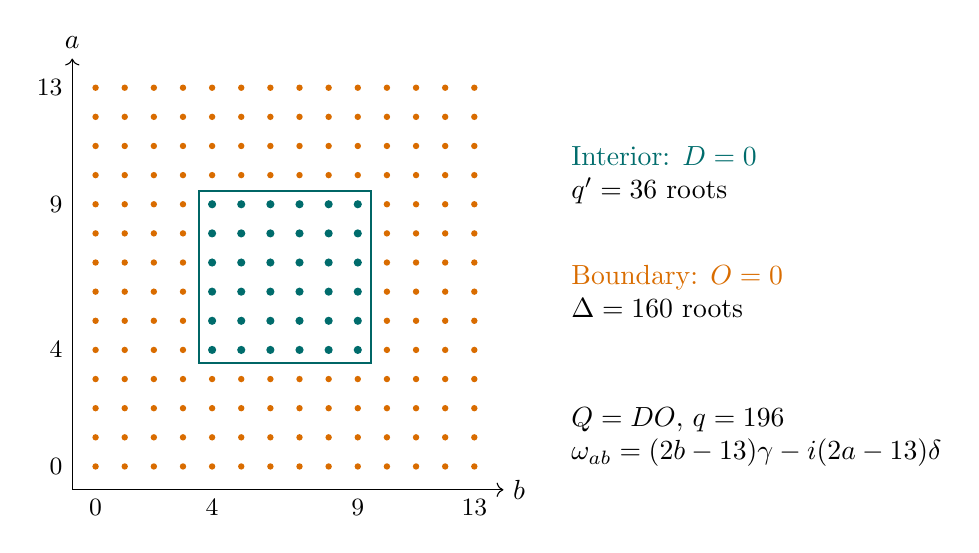
\begin{tikzpicture}[scale=.37]
\foreach \a in {0,...,13}{\foreach \b in {0,...,13}{
\ifnum\a>3\ifnum\a<10\ifnum\b>3\ifnum\b<10
\fill[teal!85!black](\b,\a)circle(.14);
\else\fill[orange!85!black](\b,\a)circle(.11);\fi
\else\fill[orange!85!black](\b,\a)circle(.11);\fi
\else\fill[orange!85!black](\b,\a)circle(.11);\fi
\else\fill[orange!85!black](\b,\a)circle(.11);\fi}}
\draw[->](-.8,-.8)--(14,-.8)node[right]{$b$};
\draw[->](-.8,-.8)--(-.8,14)node[above]{$a$};
\foreach \j in {0,4,9,13}{\node[below]at(\j,-.8){\small\j};\node[left]at(-.8,\j){\small\j};}
\draw[teal!80!black,thick](3.55,3.55)rectangle(9.45,9.45);
\node[anchor=west,align=left]at(16,10){\textcolor{teal!85!black}{Interior: $D=0$}\\$q'=36$ roots};
\node[anchor=west,align=left]at(16,6){\textcolor{orange!85!black}{Boundary: $O=0$}\\$\Delta=160$ roots};
\node[anchor=west,align=left]at(16,1){$Q=DO$, $q=196$\\$\omega_{ab}=(2b-13)\gamma-i(2a-13)\delta$};
\end{tikzpicture}
\caption{Exact index diagram for the algebraic sample $k=13$ and pivot
$(r_*,s_*)=(4,4)$. The axes are the integer indices, not the complex-plane
distance. This sample illustrates IC2--8; it is not an assertion that
IC19's eventual analytic guards hold at $k=13$. The conductor pivot
forces $x_{\mathcal I}=Fx_\partial$ on the actual kernel, proving
$K\cap\ker D(M)=0$.}
\end{figure}
\[
\begin{array}{ccc}
I_Kc&\xrightarrow{D(M)}&[D P_Kc]\\
\downarrow\pi_\partial&&\downarrow[D p]\mapsto[p]_O\\
J_\partial c&&[P_Kc]_O
\end{array}
\]
The left target uses the attained boundary metric $G_N^\partial$.
The right target uses the complete source $|D|^2d\mu_k$ at degree
$N-q'$. The exact cost of the original conductor-zero section is
$\log\det(I+\Xi_N^*\Xi_N)$ (IC35--38). No isometry is inserted.
\clearpage
\section*{Every added coefficient and every complete relation}
\addcontentsline{toc}{section}{Every added coefficient and every complete relation}
The original moment matrix and the complete row matrix grow by one
column at each cutoff. Their Schur complements give
\[
C_M=C_{M-1}+f_Mf_M^*/\nu_M,\qquad
s_M=f_M^*C_{M-1}^{-1}f_M/\nu_M\ge0.
\]
The new complete relation has squared distance $\rho_L$ from all earlier
relations, and leading coefficient $a_L=\mu_v\binom{q+L}{v}$.
The original kernel loses the exact volume factor
\[
d_L=\frac{\rho_L}{|a_L|^2\nu_{g+L}(1+s_{g+L})}\ge1.
\]
CL13--14 also identifies its precise energy content: $d_L$ is one plus
the new relation's energy in the original residual kernel divided by
its new source energy plus its observed energy. Every projection uses
the old attained metric $Q_{L-1}$.
\begin{figure}[ht]\centering
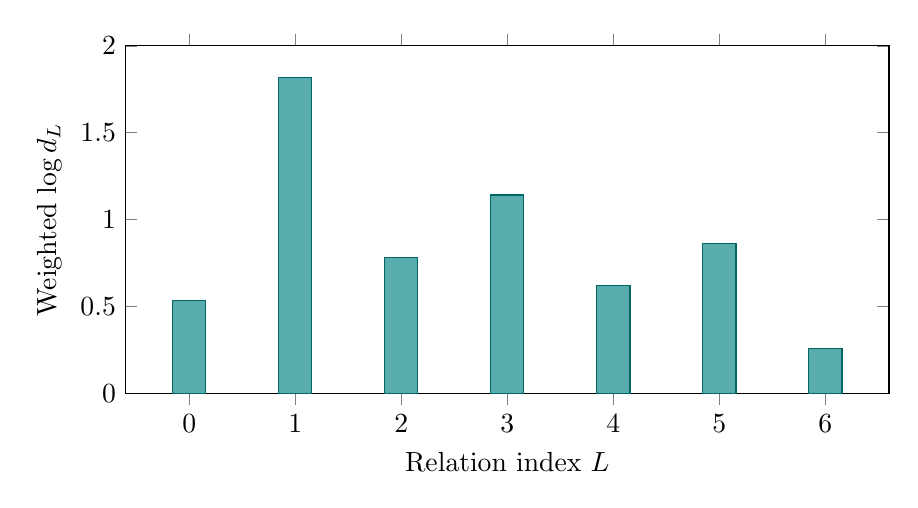
\begin{tikzpicture}
\begin{axis}[ybar,width=.93\textwidth,height=6cm,xlabel={Relation index $L$},
ylabel={Weighted $\log d_L$},xtick={0,1,2,3,4,5,6},ymin=0,
enlarge x limits=.10,bar width=12pt]
\addplot[fill=teal!65,draw=teal!80!black] coordinates {(0,0.5332747744292852) (1,1.8198077904206769) (2,0.7836306593710786) (3,1.1416701107607643) (4,0.6202793760270062) (5,0.8650296194753976) (6,0.25705454609058825)};
\end{axis}\end{tikzpicture}
\caption{Exact auxiliary complex-shift example CI26, shown with
decimal heights. The four original signs give weights $1,2,2,2,2,2,1$;
their sum is the full graph-kernel return $6.0207468765\ldots$.
All two observation rows and seven complete relation columns are present.
CI14--16 proves positivity and the exact sum. The rational factors are
retained in the executed checker receipt. This is not a native zero packet.}
\end{figure}
The finite source map underlying these calculations is KF1--55 and
CG29--32, with its complete physical comparison carried forward.
The scalar reference is evaluated by integer Hankel condensation
(CI17--24), using the identity in Christian Krattenthaler,
\emph{Advanced Determinant Calculus}, Section 2.3,
\href{https://arxiv.org/abs/math/9902004v3}{arXiv:math/9902004v3}.
\clearpage

\clearpage\part{The complete finite invariant determinant}
\section{Complete finite invariant determinant calculation}\label{complete-finite-invariant-determinant-calculation}

The complete received argument is retained below, with the sharper same-source width in equation (12), the constant-one projection estimate in equation (21), and the weighted-functional correction in the auxiliary example. The following FI sections give the additional proofs and full source identifications.

\subsection{A quantitative calculation of the original invariant determinant}\label{a-quantitative-calculation-of-the-original-invariant-determinant}

The remaining quantity is still

\[
\mathcal K_k
=
\mathcal R\log\det(I_K^*G_NI_K),
\qquad
\mathcal R f_N=f_{q-1}+f_q-f_{2q-1}-f_{2q}.
\]

The new KG, MF, and PC results do not assign its \(kq\) coefficient. The received invariant-determinant argument identifies the full projected invariant covariance as the remaining calculation.

The result obtained here is a \textbf{finite-\(k\) formula for this original determinant with an explicit \(O_{h,A}(q\log q)\) remainder}. It retains every invariant row and every lower-root projection. Its scalar reference factor is a specified positive rational number; its remaining matrix can be calculated on one fixed zero-free circle, without deleting conductor-pole rows.

In particular, the normalized remainder is

\[
O_{h,A}\!\left(\frac{\log q}{k}\right).
\]

This is a quantitative remainder for the actual kernel allocation. \textbf{The limiting coefficient remains unevaluated:} the period-dependent projected covariance in the formula below has not been numerically evaluated in this finite derivation.

The received argument used the mathematical edition at \nolinkurl{cb9705da84d6f8689611914ed9659298e620ba0a} and its checked successor \nolinkurl{bee43be41d2f6f872869d5e258fa5f752335a5ad}. The latter's recorded change is the publication-link update, not a new kernel-coefficient theorem.

\begin{center}\rule{0.5\linewidth}{0.5pt}\end{center}

\subsection{\texorpdfstring{1. The finite-\(k\) theorem}{1. The finite-k theorem}}\label{the-finite-k-theorem}

Retain

\[
q=(k+1)^2,\qquad q'=(k-7)^2,\qquad
c=k/2,\qquad c'=c-4,
\]

the original conductor order \(v\), and

\[
g=q-q'-v.
\]

At each original cutoff put

\[
L=N-q,\qquad D_N=N-v,\qquad M_N=L+g.
\]

Thus the four values of \(L\) are exactly

\[
-1,\quad0,\quad q-1,\quad q.
\]

Let \(Z\) be a complete independent row basis in the original strip coordinates, after the CG29--30 low-degree constraint elimination. Its weighted functionals have initial coefficient matrix \(A_R\); its full upper-root row embedding is \(\widetilde Z=ZS_k^{\mathsf T}\), as proved in FI2 below. Its rank is

\[
r=g-(m-s_k)=8k-32-v+s_k,
\qquad s_k=\dim(K\cap\mathcal P_{<v}).
\]

Write

\[
R_Z=ZZ^*>0,\qquad Z^\circ=R_Z^{-1/2}Z.
\]

This is an explicit, cutoff-independent change of row coordinates. Its determinant cancels under the four prescribed signs; it does not change the physical source metric.

For a row \(z\) of \(Z^\circ\), keep

\[
F_z(w)=\sum_\alpha z_\alpha e^{\beta_\alpha w},
\qquad
G_z(w)=\frac{F_z(w)}{E_A(w)},
\]

\[
H_z(t)
=(1+t^2)^{-1/4}e^{-c'w(t)}G_z(w(t)),
\qquad w(t)=-i\arctan t.
\]

The source proves that these are the actual invariant functionals, and that their covariance is

\[
C_N
=
W_NP_NW_N^*,
\qquad
P_N=I-E_N^*(E_NE_N^*)^{-1}E_N,
\tag{1}
\]

where \(E_N\) evaluates at \textbf{all} original lower roots. This is the matrix specified in the received argument, now in the fixed \(R_Z\)-orthonormal row frame.

Define the rational moments

\[
\nu_{2j}=(2j)![t^{2j}](\cos t)^{-1/2},
\qquad \nu_{2j+1}=0,
\]

and the positive rational determinants

\[
\Delta_n(a)=
\det[\nu_{2a+i+j}]_{i,j=0}^{n},
\qquad
\Delta_{-1}(a)=1.
\]

Set

\[
\boxed{
\mathcal A_{k,v}
=
\frac{
\Delta_{g-1}(q')\Delta_g(q')
\Delta_{q-1}(q-v)\Delta_q(q-v)
}{
\Delta_{q+g-1}(q')\Delta_{q+g}(q')
\Delta_0(q-v)
}.
}
\tag{2}
\]

Every factor is positive. Only moments through order \(4q-2v\) occur.

\textbf{Theorem.} On the original finite KF/CG guard domain, there is the explicitly specified error \(\mathcal E_k\) in equation (13) below such that

\[
\boxed{
\left|
\mathcal K_k
-\log\mathcal A_{k,v}
-\mathcal R\log\det C_N
\right|
\le \mathcal E_k,
\qquad
\mathcal E_k=O_{h,A}(q\log(q+2)).
}
\tag{3}
\]

Furthermore, all four \(C_N\) can be approximated using every original row, with no pole-filtration deletion, by positive matrices \(\widehat C_N\) satisfying

\[
\boxed{
\left|
\mathcal K_k
-\log\mathcal A_{k,v}
-\mathcal R\log\det\widehat C_N
\right|
\le
\mathcal E_k+\frac{4r}{4q-1}.
}
\tag{4}
\]

The required number of circle samples at each cutoff is

\[
O_{h,A}(q\log(q+2)),
\]

with an explicit sufficient count in equation (22). The absolute tolerances on the assembled original function samples and lower-root matrix require \(O_{h,A}(q\log q)\) digits in the logarithmic sense made precise below.

Equation (3) does \textbf{not} use the high-endpoint monic-profile or zero-law asymptotic. Its inputs are the finite original-source comparison, the complete conductor graph estimate, and full-polynomial Gamma inequalities. The previously obtained \(gqC_\partial\) is replaced here by the exact finite rational expression \(\log\mathcal A_{k,v}\), not by a newly asserted rate of convergence to that constant.

\subsection{2. Derivation of the scalar factor and its remainder}\label{derivation-of-the-scalar-factor-and-its-remainder}

Let

\[
d_A=\mathcal U_A1,\qquad
a_A=\mu_v\binom qv,
\]

so \(d_A\) is the full original outer polynomial of degree \(g\), with its actual leading coefficient \(a_A\).

For a polynomial \(F\), define the physical Gamma Gram

\[
\mathsf H_n[F]_{ij}
=
\int_{\mathbb R}
\overline{(c'+iy)^i}(c'+iy)^j
|F(c'+iy)|^2\,d\sigma(y),
\quad 0\le i,j\le n,
\tag{5}
\]

where

\[
d\sigma(y)=
\frac{|\Gamma(1/4+iy/2)|^2}{2\pi}\,dy,
\qquad
\mathfrak m_\sigma=\sqrt{2\pi}.
\]

An empty Gram has determinant one.

\subsubsection{The exact outer quotient determinant}\label{the-exact-outer-quotient-determinant}

The coefficient basis

\[
1,S',\ldots,S'^{g-1},
d_A,S'd_A,\ldots,S'^Ld_A
\]

has determinant \(a_A^{L+1}\). Taking its full Gram determinant and Schur-complementing the \textbf{entire} \(d_A\mathcal P_L\) relation space gives

\[
\boxed{
\det Q_N^d
=
|a_A|^{2(L+1)}
\frac{\det\mathsf H_{M_N}[\chi']}
{\det\mathsf H_L[\chi'd_A]}.
}
\tag{6}
\]

For \(L=-1\), the exponent is zero and the denominator is the empty determinant.

The source's exact complementary identity is

\[
\det H_{\overline K,Y_N}
=
|\det T_{\mathrm{frame}}|^2
\det Q_N^U\,\det C_N^U.
\]

The same fixed frame is used at every cutoff. The finite native-to-graph comparison is KF49, and the full-volume graph comparison is CG24. Consequently

\[
\boxed{
\left|
\mathcal K_k-
\mathcal R\bigl(\log\det Q_N^d+\log\det C_N\bigr)
\right|
\le
B_{\mathrm{KF49}}+\sum_NE_N^{\mathrm{vol}}.
}
\tag{7}
\]

There is no replacement of the restriction to \(\overline K\) by a full-volume estimate in this step: the actual invariant covariance \(C_N\) remains in the determinant identity.

\subsubsection{Replace the scalar reference integrals, with their full error}\label{replace-the-scalar-reference-integrals-with-their-full-error}

Use the original finite form bounds CG18 and CG20:

\[
e^{-E_{\chi'}}
\|y^{q'}p(c'+iy)\|_\sigma^2
\le
\|\chi'p\|_{\sigma,c'}^2
\le
e^{E_{\chi'}}
\|y^{q'}p(c'+iy)\|_\sigma^2,
\]

\[
e^{-E_{d,N}}|a_A|^2
\|y^{q-v}h(c'+iy)\|_\sigma^2
\le
\|\chi'd_Ah\|_{\sigma,c'}^2
\le
e^{E_{d,N}}|a_A|^2
\|y^{q-v}h(c'+iy)\|_\sigma^2.
\tag{8}
\]

Here \(p\) ranges through the complete degree-\(M_N\) space, and \(h\) through degree \(L\). The published finite bounds satisfy

\[
E_{\chi'}=O_A(1),
\qquad E_{d,N}=O_A(\log(q+2)).
\]

Their proof retains both integration regions and all exceptional outer roots; those factors are consumed through their displayed errors, not removed.

Define

\[
\mathsf J_n^{(a)}
=
\left[\int y^{2a+i+j}\,d\sigma(y)\right]_{i,j=0}^n.
\]

The transformation from \(S'^j=(c'+iy)^j\) to \(y^j\) is triangular with diagonal \(i^j\). Its determinant has modulus one. Thus (8), followed by determinants in the same coefficient frames, gives

\[
\boxed{
\left|
\log\det Q_N^d
-
\left[
\log\det\mathsf J_{M_N}^{(q')}
-\log\det\mathsf J_L^{(q-v)}
\right]
\right|
\le
(M_N+1)E_{\chi'}+(L+1)E_{d,N}.
}
\tag{9}
\]

The factor \(|a_A|^{2(L+1)}\) in (6) cancels the identical factor in the full relation Gram. This is the exact location of that cancellation.

The Gamma generating function, in the retained monic convention, is

\[
\sum_{n\ge0}\frac{p_n(y)}{n!}t^n
=
(1+t^2)^{-1/4}e^{y\arctan t}.
\]

Integrating its formal coefficients and then putting \(t=\tan u\) gives

\[
\boxed{
\sum_{j\ge0}\frac{u^j}{j!}
\int y^j\,d\sigma(y)
=
\mathfrak m_\sigma(\cos u)^{-1/2}.
}
\tag{10}
\]

This follows from the Meixner--Pollaczek generating function in the original variable and normalization; no probability normalization has been imposed. (\href{https://dlmf.nist.gov/18.23.E7}{DLMF})

Hence

\[
\det\mathsf J_n^{(a)}
=
\mathfrak m_\sigma^{\,n+1}\Delta_n(a).
\]

At each cutoff, the difference in dimensions in (9) is \(g\). Its mass term is therefore \(g\log\mathfrak m_\sigma\), whose four-cutoff return is exactly zero. Substituting the four values of \(L\) yields precisely

\[
\boxed{
\mathcal R
\left[
\log\det\mathsf J_{M_N}^{(q')}
-\log\det\mathsf J_L^{(q-v)}
\right]
=\log\mathcal A_{k,v}.
}
\tag{11}
\]

For reference, the first normalized moments are

\[
1,\quad \frac12,\quad \frac74,\quad
\frac{139}{8},\quad \frac{5473}{16}
\]

in even orders \(0,2,4,6,8\). Odd orders vanish. All later moments in (2) are obtained by the same exact power series.

\subsubsection{The complete finite remainder}\label{the-complete-finite-remainder}

The retained source bound is

\[
B_{\mathrm{KF49}}
=
2m\Lambda_k
+2s_k\log\kappa_k^*
+2B_k^{\mathrm{ang}}
+2\sum_NE_N^*,
\]

where

\[
B_k^{\mathrm{ang}}
=
v\log\kappa_k^*
+2v\log(1/\varepsilon_k),
\]

\[
E_N^*=(N+1)\log M_{N-v}+J_{N-v},
\qquad
J_D=(D+1)\log^+(1/|(-i)^v\mu_v/v!|).
\tag{12}
\]

These are the original finite interpolation, low-angle, and exterior constants in KF37--49. The graph error \(E_N^{\mathrm{vol}}\) is zero at both low cutoffs and is the full CG24 bound at the high cutoffs.

Thus the error in (3) is explicitly

\[
\boxed{
\mathcal E_k
=
B_{\mathrm{KF49}}
+\sum_N
\left[
E_N^{\mathrm{vol}}
+(M_N+1)E_{\chi'}
+(L+1)E_{d,N}
\right].
}
\tag{13}
\]

Every term is a previously specified finite source quantity. Since

\[
M_N=O(q),\quad L+1\le q+1,\quad m=O(k),
\]

their proved orders give

\[
\mathcal E_k=O_{h,A}(q\log(q+2)).
\]

This is a bound around a finite determinant formula. It is not a claim that the unresolved invariant covariance already has a limiting coefficient.

\subsection{3. Every original invariant row can be calculated on one fixed circle}\label{every-original-invariant-row-can-be-calculated-on-one-fixed-circle}

The existing CGP sampling construction works near the unit circle after imposing conductor-pole cancellation conditions on a smaller row space. The following construction keeps \textbf{all} rows. Its circle is chosen inside a certified zero-free neighborhood of the original symbol.

Write

\[
E_A(w)=\sum_{j=1}^{J}a_je^{b_jw},
\qquad
v=\operatorname{ord}_0E_A,
\qquad
\mu_v=E_A^{(v)}(0)\ne0.
\]

Set

\[
A_1=\sum_j|a_j|,
\qquad B_A=\max(1,\max_j|b_j|),
\qquad
C_v=\frac{A_1B_A^v}{|\mu_v|}.
\]

Define

\[
R_A=
B_A^{-1}
\min\left(1,\frac{v+1}{2eC_v}\right),
\qquad
s=R_A/2,\qquad a=s/2.
\tag{14}
\]

These depend on the fixed actual conductor, not on \(k\).

Taylor's formula gives, for \(|w|\le R_A\),

\[
\left|
\frac{v!E_A(w)}{\mu_vw^v}-1
\right|
\le
C_v\frac{B_A|w|e^{B_A|w|}}{v+1}
\le\frac12.
\]

Therefore

\[
\boxed{
|E_A(w)/w^v|\ge\frac{|\mu_v|}{2v!}.
}
\tag{15}
\]

At \(w=0\), the quotient denotes its removable value.

Let

\[
R_k=k\sqrt{\delta^2+\gamma^2},
\qquad B_k=4+R_k,
\qquad n_E=16k-48.
\]

For every coefficient-unit row in the original invariant row space,

\[
e^{-c'w}F_z(w)
=\sum_\alpha z_\alpha e^{(\beta_\alpha-c')w}
\]

vanishes through order \(v-1\), has at most \(n_E\) nonzero terms, and

\[
|\beta_\alpha-c'|\le B_k.
\]

Hence

\[
\left|
w^{-v}e^{-c'w}F_z(w)
\right|
\le
\frac{\sqrt{n_E}B_k^v}{v!}e^{B_k|w|}.
\]

For \(|t|\le s\le1/2\),

\[
|w(t)|\le\operatorname{arctanh}s<R_A.
\]

Combining this with (15),

\[
\boxed{
|H_z(t)|\le A_k\|z\|_2,
\qquad
A_k=
\frac{2\sqrt{n_E}B_k^v}{|\mu_v|}
(1-s^2)^{-1/4}
e^{B_k\operatorname{arctanh}s}.
}
\tag{16}
\]

Thus \(H_z\) is holomorphic on the entire disk \(|t|\le s\), for every original row, and

\[
\log A_k=O_{h,A}(k+\log(k+2)).
\]

No zero of \(E_A\) outside this disk is omitted from the function: it remains encoded in its Taylor coefficients.

\subsubsection{Exact aliasing formula}\label{exact-aliasing-formula}

Put

\[
\rho_n=\sqrt{\frac{n!}{(1/2)_n}},
\qquad
(W_N)_{z,n}
=
\frac{\rho_n}{\sqrt{\mathfrak m_\sigma}}[t^n]H_z(t),
\quad 0\le n\le D_N.
\]

Define

\[
B_N=
\max\left\{
1,\,
\frac{A_k}{\sqrt{\mathfrak m_\sigma}}
\left(\sum_{n=0}^{D_N}\rho_n^2s^{-2n}\right)^{1/2}
\right\}.
\tag{17}
\]

Then \(\|W_N\|\le B_N\).

For \(T>D_N\), let \(\omega_T=e^{2\pi i/T}\), and calculate

\[
[t^n]^{[T]}H_z
=
\frac{a^{-n}}T
\sum_{\ell=0}^{T-1}
H_z(a\omega_T^\ell)\omega_T^{-n\ell}.
\]

Writing \(H_z(t)=\sum c_jt^j\), the exact discrete Fourier identity is

\[
[t^n]^{[T]}H_z-c_n
=
\sum_{j\ge1}c_{n+jT}a^{jT}.
\]

Since \(a/s=1/2\), Cauchy's coefficient estimate yields the full matrix bound

\[
\boxed{
\|W_N^{[T]}-W_N\|
\le
B_N\frac{2^{-T}}{1-2^{-T}}.
}
\tag{18}
\]

The bound holds simultaneously on every linear combination of the original rows.

\subsection{4. The lower-root projection has an explicit precision budget}\label{the-lower-root-projection-has-an-explicit-precision-budget}

Let \(a_*\) be the actual leading biform conductor coefficient from OCF5, and put

\[
\kappa_A=A_1/|a_*|.
\]

The full original strip reduction has path length at most \(10k\). The source consequently proves

\[
C_N\succeq\lambda_N I_r,
\]

where a valid finite choice is

\[
\boxed{
\lambda_N
=
\min\left\{
1,\,
\left[
M_{D_N}^2 B_{\mathrm{val}}q\kappa_A^{20k}
\right]^{-1}
\right\},
}
\tag{19}
\]

\[
B_{\mathrm{val}}
=
q\mathfrak m_\sigma
\left(\frac{2q+R_k}{2\delta}\right)^{2(q-1)}.
\]

Here \(M_{D_N}\ge1\) is the unchanged full-conductor forward bound. In particular,

\[
\log(1/\lambda_N)=O_{h,A}(q\log(q+2)).
\]

This is the lower bound \textbf{after} the full lower-root projection, not the easier unprojected strip bound.

For the lower-root matrix itself, the complete lower Lagrange polynomials give

\[
\sigma_{\min}(E_N)\ge s_E,
\]

with

\[
\boxed{
s_E=
\left[
q'\mathfrak m_\sigma
\left(\frac{2q'+R_-}{2\delta}\right)^{2(q'-1)}
\right]^{-1/2},
\qquad
R_-=(k-8)\sqrt{\delta^2+\gamma^2}.
}
\tag{20}
\]

Indeed the coefficient columns of those interpolation polynomials form a right inverse of \(E_N\); the sum of their squared Gamma norms bounds its squared operator norm.

If

\[
\|\widehat E_N-E_N\|\le\epsilon_E\le s_E/2,
\]

the full row rank persists, and

\[
\boxed{
\|\widehat P_N-P_N\|\le\epsilon_E/s_E,
}
\tag{21}
\]

where \(\widehat P_N\) is formed using every row of \(\widehat E_N\). The equal-rank principal-angle proof in FI5 establishes the constant-one estimate (21).

Choose \(0<\theta\le1/2\), and set

\[
\boxed{
T_N=
\max\left\{
D_N+1,\,
\left\lceil
\log_2\frac{32B_N^2}{\theta\lambda_N}
\right\rceil
\right\}.
}
\tag{22}
\]

Require the additional row-evaluation error to satisfy

\[
\|\widehat W_N-W_N^{[T_N]}\|
\le\frac{\theta\lambda_N}{16B_N},
\]

and require

\[
\boxed{
\|\widehat E_N-E_N\|
\le
\frac{\theta\lambda_Ns_E}{32B_N^2}.
}
\tag{23}
\]

Equation (18) gives

\[
e_N:=\|\widehat W_N-W_N\|
\le\frac{\theta\lambda_N}{8B_N}.
\]

Therefore

\[
\begin{aligned}
\|\widehat W_N\widehat P_N\widehat W_N^*
-W_NP_NW_N^*\|
&\le (2B_N+e_N)e_N\\
&\quad +(B_N+e_N)^2\|\widehat P_N-P_N\|\\
&<\theta\lambda_N.
\end{aligned}
\]

Thus

\[
\boxed{
(1-\theta)C_N
\preceq\widehat C_N
\preceq(1+\theta)C_N.
}
\tag{24}
\]

The final products and inverses can be performed exactly on Gaussian-rational centers, or their additional arithmetic error must be included in the displayed margin. A floating-point midpoint is not by itself a certificate.

For \(\theta=1/(4q)\), the four correlated determinant errors satisfy

\[
\boxed{
|\mathcal R\log\det\widehat C_N
-\mathcal R\log\det C_N|
\le
2r\log\frac{4q+1}{4q-1}
\le\frac{4r}{4q-1}.
}
\tag{25}
\]

Equations (3) and (25) prove (4).

Because \(s,a\) are fixed by the actual conductor,

\[
\log B_N=O_{h,A}(q),
\qquad
\log(1/s_E)=O_h(q\log q).
\]

It follows directly from (22)--(23) that the sample count and logarithmic absolute tolerances have the claimed \(O_{h,A}(q\log q)\) sizes.

These are tolerances on the \textbf{assembled original row functions and lower-root evaluations}. Additional uncertainty in a period, physical unit, or selected invariant frame must be propagated into them; the theorem does not invent such input enclosures.

\subsubsection{Evaluating the removable quotient without cancellation}\label{evaluating-the-removable-quotient-without-cancellation}

The samples need not be calculated by dividing two tiny raw values. Write

\[
w^{-v}e^{-c'w}F_z(w)=\sum_{\ell\ge0}f_{z,\ell}w^\ell,
\qquad
w^{-v}E_A(w)=\sum_{\ell\ge0}g_\ell w^\ell.
\]

Their exact coefficients are

\[
f_{z,\ell}
=
\frac{\sum_\alpha z_\alpha(\beta_\alpha-c')^{v+\ell}}
{(v+\ell)!},
\qquad
g_\ell=\frac{\mu_{v+\ell}}{(v+\ell)!}.
\]

The quotient coefficients satisfy

\[
\boxed{
u_{z,0}=f_{z,0}/g_0,\qquad
u_{z,n}
=
g_0^{-1}
\left(
f_{z,n}-\sum_{j=1}^ng_ju_{z,n-j}
\right).
}
\tag{26}
\]

All zero coefficients below order \(v\) are enforced by the original algebraic constraints.

For example, truncation after \(\ell=L-1\) has the explicit numerator tail

\[
\left|
\sum_{\ell\ge L}f_{z,\ell}w^\ell
\right|
\le
\sqrt{n_E}\|z\|_2 B_k^v
\frac{(B_k|w|)^Le^{B_k|w|}}{(v+L)!},
\tag{27}
\]

and the analogous denominator tail replaces \(\sqrt{n_E}B_k^v\) by \(A_1B_A^v\). The denominator floor is already (15).

Thus the new precision statement includes a convergent, guarded calculation of the actual samples; it does not assume that a black-box evaluation of \(F_z/E_A\) is stable.

\subsection{5. An algebraic route uses the actual invariant rows as initial data}\label{an-algebraic-route-uses-the-actual-invariant-rows-as-initial-data}

There is also a finite coefficient calculation of the same projected covariance, with no Cauchy sampling.

Let

\[
\ell_z[\eta]
=
[\eta(\partial_w)\chi'(\partial_w)G_z(w)]_{w=0},
\]

and write

\[
u_n(S')
=
\mathcal U_A(S^n)(S')
=
\sum_j a_jd_j(S')(S'+b_j)^n.
\]

The source's full relation identity proves

\[
\ell_z[u_n]=0.
\]

Moreover,

\[
\deg u_n=n+g,
\qquad
[S'^{n+g}]u_n
=
\mu_v\binom{q+n}{v}\ne0.
\]

Hence the actual moments

\[
b_{z,j}=\ell_z[S'^j]
\]

satisfy the exact triangular recurrence

\[
\boxed{
b_{z,n+g}
=
-\frac{
\sum_{j=0}^{n+g-1}[S'^j]u_n\,b_{z,j}
}{
\mu_v\binom{q+n}{v}
}.
}
\tag{28}
\]

The first \(g\) columns are precisely the original \(A_R\), with its low-constraint elimination. No free initial row is inserted.

Let \(\mathsf B_N=[b_{z,j}]_{j=0}^{M_N}\). Multiplication by the full \(\chi'\) has a coefficient matrix \(J_{\chi',N}\) into the lower Gamma-orthonormal frame, satisfying

\[
J_{\chi',N}^*J_{\chi',N}
=\mathsf H_{M_N}[\chi'],
\]

\[
P_N
=
J_{\chi',N}
\mathsf H_{M_N}[\chi']^{-1}
J_{\chi',N}^*,
\qquad
\mathsf B_N=W_NJ_{\chi',N}.
\]

Therefore

\[
\boxed{
C_N
=
\mathsf B_N\mathsf H_{M_N}[\chi']^{-1}\mathsf B_N^*.
}
\tag{29}
\]

This is a factorization of the \textbf{full lower-root projection}, not its replacement by the identity.

It gives a useful complete bordered determinant. Set

\[
\mathbb H_N=
\begin{pmatrix}
\mathsf H_{M_N}[\chi']&\mathsf B_N^*\\
\mathsf B_N&0
\end{pmatrix},
\]

\[
\mathsf R_N
=
\mathsf U_N^*
\mathsf H_{M_N}[\chi']
\mathsf U_N,
\]

where \(\mathsf U_N\) contains all relation columns

\[
u_0,u_1,\ldots,u_L,
\]

and

\[
\tau_N=\prod_{n=0}^{L}\mu_v\binom{q+n}{v}.
\]

Empty products and empty relation determinants equal one.

The complete graph basis has determinant \(\tau_N\). Block elimination gives

\[
(-1)^r\det\mathbb H_N
=
\det\mathsf H_{M_N}[\chi']\det C_N>0.
\]

Consequently

\[
\boxed{
\left|
\mathcal K_k
-
\mathcal R\log
\left[
\frac{
|\tau_N|^2(-1)^r\det\mathbb H_N
}{
\det\mathsf R_N
}
\right]
\right|
\le B_{\mathrm{KF49}}.
}
\tag{30}
\]

Equation (30) retains the \textbf{original nonideal relation operator \(\mathcal U_A\)}. It requires no passage from its graph to the outer ideal. In particular, the large source determinant cancels exactly inside the bordered formula; the complete relation Gram in the denominator remains.

Equations (28)--(30) and the all-row Cauchy construction are two independent ways to calculate the same actual invariant covariance. Their equality supplies an exact cross-check for an implementation.

\subsection{6. What the rational quotient does to these actual rows}\label{what-the-rational-quotient-does-to-these-actual-rows}

The allowed quotient must be carried through the lower-root projection before any minimization. That transport can be written explicitly.

Let \(\mathcal D\) be an admitted rational denominator, and let \(U_{\mathcal D}\) be its original root-value numerator map. Put

\[
R_{\mathcal D}=C_AU_{\mathcal D}.
\]

On the MF degree guard, this has full column rank. Choose the exact coefficient left inverse

\[
L_{\mathcal D}
=
(R_{\mathcal D}^*R_{\mathcal D})^{-1}R_{\mathcal D}^*,
\]

and define

\[
B_{\mathcal D}
=
\widetilde ZU_{\mathcal D}L_{\mathcal D},
\qquad
Z_{\mathcal D}=\widetilde Z-B_{\mathcal D}C_A.
\tag{31}
\]

Then

\[
Z_{\mathcal D}U_{\mathcal D}=0,
\]

so \(Z_{\mathcal D}\) factors through the actual \(\pi_{\mathcal D}\). Here \(\widetilde Z=ZS_k^{\mathsf T}\) is the full upper-root row matrix. The coefficient left inverse in (31) is used only to specify the map; it is not declared an isometry of a native metric.

Each row of \(C_A\), at a lower root \(\eta\), has exponential numerator

\[
E_A(w)e^{\eta w}.
\]

Therefore

\[
G_{z_{\mathcal D}}(w)
=
G_z(w)-\sum_\eta(B_{\mathcal D})_{z\eta}e^{\eta w},
\]

and its Gamma row is exactly

\[
\boxed{
W_{N,\mathcal D}=W_N-B_{\mathcal D}E_N.
}
\tag{32}
\]

Since \(E_NP_N=0\),

\[
\boxed{
W_{N,\mathcal D}P_NW_{N,\mathcal D}^*
=
W_NP_NW_N^*.
}
\tag{33}
\]

This is the explicit original-row consequence of the quotient. It preserves every lower-root constraint. It also shows why choosing another admitted pole family does not by itself assign a new value to the remaining projected covariance: its projected Gram is exactly the same.

The unprojected Gram does change:

\[
W_{N,\mathcal D}W_{N,\mathcal D}^*
\ne W_NW_N^*
\]

in general. Therefore one cannot replace the strip-angle denominator by the new unprojected Gram without carrying that change separately.

At a resultant zero or observation-rank drop, (31) is not used. The PC7 and PC27 exact kernel sequences, and PC32's positive-rank determinant identity, are the applicable maps. The new off-boundary sampling estimate is not asserted through a vanishing observed fraction.

\subsection{7. An exact example retaining an interior conductor pole and the full projection}\label{an-exact-example-retaining-an-interior-conductor-pole-and-the-full-projection}

The following is a finite complex-conductor illustration of the new mechanism, \textbf{not} a native xi packet.

Take

\[
\mathcal T_Af(S')=f(S'+4i)-f(S'),
\]

\[
\chi'(S')=S'(S'-1),
\]

\[
\chi(S)=S(S-1)(S-4i)(S-1-4i).
\]

Choose the upper row

\[
F_z(w)=e^w-1.
\]

Then

\[
E_A(w)=e^{4iw}-1,\qquad
G_z(w)=\frac{e^w-1}{e^{4iw}-1}.
\]

Its first coefficients are

\[
G_z(w)
=
-\frac i4
+\left(-\frac12-\frac i8\right)w
+\left(-\frac14+\frac{7i}{24}\right)w^2+\cdots.
\]

At \(N=3\), the lower Gamma degree is \(2\). In the original Gamma-orthonormal frame,

\[
W=
\frac1{\sqrt{\mathfrak m_\sigma}}
\left(
-\frac i4,\,
\sqrt2\left(-\frac18+\frac i2\right),\,
\sqrt{\frac23}\left(\frac12-\frac{11i}{24}\right)
\right),
\]

and the two original lower-root evaluation rows are

\[
E=
\frac1{\sqrt{\mathfrak m_\sigma}}
\begin{pmatrix}
1&0&-1/\sqrt6\\
1&-i\sqrt2&-\sqrt{3/2}
\end{pmatrix}.
\]

Directly,

\[
WW^*=\frac{389}{432\mathfrak m_\sigma}.
\]

The lower-root ideal is spanned by

\[
\chi'(iy)=-y^2-iy,
\]

whose squared norm is

\[
\|\chi'\|_\sigma^2=\frac94\mathfrak m_\sigma.
\]

The actual functional value is

\[
L_z[\chi']=\ell_z[1]=G_z''(0)-G_z'(0)=\frac{17i}{24}.
\]

Thus

\[
\boxed{
WP_IW^*
=
\frac{289}{1296\mathfrak m_\sigma},
\qquad
\frac{WP_IW^*}{WW^*}
=
\frac{289}{1167}.
}
\tag{34}
\]

The generating function has an actual interior pole at

\[
t=i\tanh(\pi/2),
\]

because \(w(t)=\pi/2\), the denominator vanishes there, and the numerator does not. The fixed circle in (14) lies inside that pole and computes this full row without deleting it.

Equation (34) independently agrees with the algebraic formula (29), where the weighted source Gram has the single entry \(9\mathfrak m_\sigma/4\). Omitting the lower-root projection would replace \(289/1296\) by \(389/432\), a different covariance.

\subsection{8. Consequences for the outstanding coefficient}\label{consequences-for-the-outstanding-coefficient}

The complete finite approximation is now

\[
\boxed{
\frac{\mathcal K_k}{kq}
=
\frac{
\log\mathcal A_{k,v}
+\mathcal R\log\det\widehat C_N
}{kq}
+
O_{h,A}\!\left(\frac{\log(q+2)}k\right),
}
\tag{35}
\]

with the finite error given by (13), (22)--(25), rather than an unspecified asymptotic remainder.

The full invariant covariance is increasing with the allowed source degree. Thus

\[
\mathcal R\log\det C_N\le0.
\]

The original kernel metric decreases with the source degree, so

\[
\mathcal K_k\ge0.
\]

Equations (3) and (11) therefore also give the finite upper bound

\[
\boxed{
0\le\mathcal K_k
\le\log\mathcal A_{k,v}+\mathcal E_k.
}
\tag{36}
\]

Using the separately established outer-volume limit would yield

\[
\limsup\frac{\mathcal K_k}{kq}\le16C_\partial.
\]

That is only an upper bound; it is not the missing coefficient.

The useful advance is more specific than that coarse bound. \textbf{The canonical kernel allocation now has an all-row, full-projection finite calculation with an \(O(q\log q)\) physical comparison error and an independently adjustable numerical determinant error.} There is no complementary pole-row determinant left to estimate. The exact quotient transport is (31)--(33), and the original nonideal relation calculation is (28)--(30).

The actual numerical sequence \(\mathcal R\log\det C_N/(kq)\), or an analytic asymptotic for those same invariant rows, remains to be evaluated. No complex-current phase is assigned by these positive Gram calculations. The exact auxiliary checks accompanying this proof verify the finite algebra. They do not evaluate the original native period-dependent covariance sequence.

\subsubsection{References}\label{references}

Koornwinder, T. H., Wong, R., Koekoek, R., Swarttouw, R. F., \& Reinhardt, W. P. (n.d.). Orthogonal polynomials. In \emph{NIST Digital Library of Mathematical Functions} (Chapter 18). Equations 18.22.8 and 18.23.7 supply the recurrence and generating-function conventions used above. (\href{https://dlmf.nist.gov/18}{DLMF})

Split-Zero research programme. (2026a, September 21). \href{https://github.com/KokunoYumeto/zeta-function-research-reader/blob/0fd693c844aad9117e30ec447c59864a28af10f3/workbenches/splitzero-tandem/continuations/20260921-native-spectral-real-pair/003/ACTUAL_KERNEL_FILTRATION_AND_GRAPH.tex\#L270}{\emph{ACTUAL\_KERNEL\_FILTRATION\_AND\_GRAPH.tex}, KF37--55}. \emph{Zeta-function research reader}, pinned original proof edition. The complete finite source comparison, relation graph, and fixed-frame determinant transport are the inherited inputs to (7) and (30).

Split-Zero research programme. (2026b, September 21). \href{https://github.com/KokunoYumeto/zeta-function-research-reader/blob/0fd693c844aad9117e30ec447c59864a28af10f3/workbenches/splitzero-tandem/continuations/20260921-native-spectral-real-pair/003/COMPLETE_CONDUCTOR_GRAPH_METRIC.tex\#L113}{\emph{COMPLETE\_CONDUCTOR\_GRAPH\_METRIC.tex}, CG18--32}. Same pinned original proof edition. The full-form errors and the post-projection lower bound are retained with their original finite domains.

\section{Additional finite proofs and exact source identifications}\label{additional-finite-proofs-and-exact-source-identifications}

\subsection{FI1. The sharper comparison on the identical source}\label{fi1.-the-sharper-comparison-on-the-identical-source}

The original simple-quartet domain has multiplicity parameter \(m_0=1\), \(k\equiv1\pmod4\), \(q=(k+1)^2\), \(c=k/2\), the unchanged divisor \(h\), and arithmetic measure \(d\mu_k=w_h^{*k}(y)\,dy\), \(w_h(y)=|(2\xi/h)(1/2+iy)|^2/(2\pi)\). This is precisely NG1 with \(m_0=1\), not a comparison with a different arithmetic model. In \href{https://github.com/KokunoYumeto/zeta-function-research-reader/blob/5992ad50c0f2a06921f1fcaded7b4e38097c0739/workbenches/splitzero-tandem/continuations/20260920-original-kernel-mixed-determinants/providers/NATIVE_GAUSSIAN_TRANSFER.tex\#L27}{NG1--3, lines 27--72}, put \(M=21+4m_0=25\) and use its original positive full-mass constants \(a_k,A_k\) from CAI16. Then, simultaneously for every original polynomial degree \(N\le2q\), \[
\begin{gathered}\ell_{k,2q}\|p\|_\sigma^2\le\|p\|_{\mu_k}^2\le u_k\|p\|_\sigma^2,\\
 \quad \ell_{k,2q}=\frac{a_k}{[1+4(2q+25)^2]^{25}},\quad u_k=A_k,
 \quad \Lambda_k=\log\frac{u_k}{\ell_{k,2q}}=O_h(k+\log(q+2)).
\end{gathered}\tag{FI1}
\] The polynomial is the full original polynomial evaluated at \(c+iy\). Its roots and its coefficient frame are unaltered. The different lower physical center \(c'=c-4\) enters only in the subsequent KF conductor transport, whose existing bounds remain.

Here is the exact passage from FI1 to an arbitrary fixed target subspace. Let \(T_N:\mathcal P_N\to V\) be the original onto coefficient map; write \(G_N^{\mu}\) and \(G_N^\sigma\) for its attained metrics. The minimum of a positive definite finite-dimensional quadratic form over the closed affine fibre \(T_Np=x\) exists: decompose the source into \(\ker T_N\) and its orthogonal complement, on which \(T_N\) is an isomorphism onto \(V\). Applying FI1 to every element of that same fibre and then taking infima gives \[
 \ell_{k,2q}G_N^\sigma\preceq G_N^\mu\preceq u_kG_N^\sigma.
 \tag{FI2}
\] For every fixed injective rank-\(t\) frame \(J:\mathbb C^t\to V\), congruence by \(J\) preserves these inequalities. Congruence again by \((J^*G_N^\sigma J)^{-1/2}\) puts every eigenvalue in \([\ell_{k,2q},u_k]\). Multiplying the eigenvalues proves \[
 t\log\ell_{k,2q}\le d_N:=\log\frac{\det(J^*G_N^\mu J)}{\det(J^*G_N^\sigma J)}\le t\log u_k.
\] There are exactly two positive and two negative signs in \(\mathcal R\). Thus the largest possible value of \(\mathcal R d_N\) is \(2t\log u_k-2t\log\ell_{k,2q}\) and the smallest is its negative. Consequently \[
 |\mathcal R d_N|\le2t\Lambda_k.\tag{FI3}
\] Use the original frame \(J=I_K\), with \(t=m=8k-16\). This proves the sharper MR21/JM25 receiver directly from the same source. It changes only the width term in \href{https://github.com/KokunoYumeto/zeta-function-research-reader/blob/0fd693c844aad9117e30ec447c59864a28af10f3/workbenches/splitzero-tandem/continuations/20260921-native-spectral-real-pair/003/ACTUAL_KERNEL_FILTRATION_AND_GRAPH.tex\#L354}{KF49, lines 354--363}: \[
 B_{\rm KF49}^{\rm sharp}=2m\Lambda_k+2s_k\log\kappa_k^*+2B_k^{\rm ang}+2\sum_NE_N^*.
 \tag{FI4}
\] Every original low intersection, angle, exterior bound, physical mass and finite guard stays in FI4. In particular \(E_N^*=(N+1)\log M_{N-v}+(N-v+1)\log^+(1/|(-i)^v\mu_v/v!|)\) is unchanged. Adding the \href{https://github.com/KokunoYumeto/zeta-function-research-reader/blob/0fd693c844aad9117e30ec447c59864a28af10f3/workbenches/splitzero-tandem/continuations/20260921-native-spectral-real-pair/003/COMPLETE_CONDUCTOR_GRAPH_METRIC.tex\#L158}{CG24 full-volume error, lines 158--192} and the \href{https://github.com/KokunoYumeto/zeta-function-research-reader/blob/0fd693c844aad9117e30ec447c59864a28af10f3/workbenches/splitzero-tandem/continuations/20260921-native-spectral-real-pair/003/COMPLETE_CONDUCTOR_GRAPH_METRIC.tex\#L113}{CG18--20 scalar errors, lines 113--136} gives exactly equation (13), with equation (12) read as FI4. Its order is \(O_{h,A}(q\log(q+2))\): the new first term is \(O_h(k^2+k\log(q+2))=O_h(q)\) and all retained terms have the stated \(O(q\log(q+2))\) bound. The former width of order \(k\log^2q\) would not prove this sharper remainder.

\subsection{FI2. Original strip rows, full upper-root rows and weighted functionals}\label{fi2.-original-strip-rows-full-upper-root-rows-and-weighted-functionals}

Let \(S_k:\mathbb C^{n_E}\to\mathbb C^q\) insert zeros in the original conductor pivot positions, in the lexicographic coefficient order of \href{https://github.com/KokunoYumeto/zeta-function-research-reader/blob/5992ad50c0f2a06921f1fcaded7b4e38097c0739/workbenches/splitzero-tandem/continuations/20260920-original-kernel-mixed-determinants/providers/ORIGINAL_CONDUCTOR_STRIP_FRAME.tex\#L34}{OCF2--8, lines 34--163}. Thus \(S_k^*S_k=I\), \(n_E=16k-48\), and a strip row \(z\) means the full upper-root row \(\widetilde z=zS_k^{\mathsf T}\). Transposition here specifies the complex-linear evaluation row; \(S_k\) is a real zero-insertion matrix, so its transpose also equals its adjoint. In particular \(\|\widetilde z\|_2=\|z\|_2\). The symbol in every equation (1)--(34) is \[
 F_z(w)=\sum_{\alpha=1}^q\widetilde z_\alpha e^{\beta_\alpha w}.
 \tag{FI5}
\] The row basis is obtained by the exact CG29--30 low-degree elimination. That elimination says \(\sum_\alpha\widetilde z_\alpha\beta_\alpha^j=0\) for \(0\le j<v\). It therefore makes \(F_z/E_A\) holomorphic at zero. It does not replace the physical norm by the Euclidean row norm. Applying \((ZZ^*)^{-1/2}\) to all rows is the same fixed invertible row map at all cutoffs, and its determinant contribution \(-\log\det(ZZ^*)\) cancels because \(1+1-1-1=0\).

Define two distinct complex-linear functionals: \[
 L_z(f)=[f(\partial_w)G_z(w)]_{w=0},\qquad
 \ell_z(\eta)=L_z(\chi'\eta),\qquad G_z=F_z/E_A.
 \tag{FI6}
\] The first has domain the unweighted lower polynomial space; the second has domain the weighted coefficient polynomial space. The Taylor identity \(E_AG_z=F_z\) implies, first on a monomial and then by linearity, \[
 L_z(\mathcal T_Ap)=\sum_\alpha\widetilde z_\alpha p(\beta_\alpha).
 \tag{FI7}
\] To verify it explicitly, \(\mathcal T_A=e^{b_1\partial}a_1+\cdots+e^{b_J\partial}a_J\). Thus \((\mathcal T_Ap)(\partial_w)G_z|_0=p(\partial_w)(E_AG_z)|_0=p(\partial_w)F_z|_0\). Only finitely many derivatives occur for each polynomial.

Let \(D=N-v\) and \(M=N-v-q'=L+g\). In the lower source use the exact orthonormal polynomials \[
 \psi_n(S')=\frac{p_n(-i(S'-c'))}{\sqrt{\mathfrak m_\sigma n!(1/2)_n}},\quad0\le n\le D.
\] Their squared norm on \(S'=c'+iy\) is one. Substituting the complete generating function gives \(L_z(\psi_n)=\rho_n[t^n]H_z/\sqrt{\mathfrak m_\sigma}\), exactly the row \(W_N\) in the retained text. Let \(E_N\) evaluate these polynomials at every lower root. The roots are distinct on the original simple-quartet domain, and \(D\ge q'-1\), so interpolation proves \(\operatorname{rank}E_N=q'\). Its kernel is exactly \(\chi'\mathcal P_M\): a degree-at-most-\(D\) polynomial vanishes at all \(q'\) distinct roots if and only if it is divisible by their full monic product. The coefficient map \(J=J_{\chi',N}\) of \(\eta\mapsto\chi'\eta\) has this range, is injective, and satisfies \(J^*J=\mathsf H_M[\chi']\). Consequently \[
 P_N=J(J^*J)^{-1}J^*,\quad W_NJ=\mathsf B_N,
 \quad C_N=\mathsf B_N\mathsf H_M[\chi']^{-1}\mathsf B_N^*.
 \tag{FI8}
\] Indeed \(J(J^*J)^{-1}J^*\) is self-adjoint, fixes the range of \(J\), and annihilates its orthogonal complement. This proves equality to the full root-kernel projection, including every original lower root.

The identity \(\mathcal T_A(\chi S^n)=\chi'u_n\) and FI7 give \(\ell_z(u_n)=0\), because \(\chi(\beta_\alpha)=0\) at every upper root. Since \(u_n\) has exact degree \(g+n\) and leading coefficient \(a_n=\mu_v\binom{q+n}{v}\ne0\), coefficient comparison gives equation (28). Inductively it determines every \(b_{z,j}\) for \(j\ge g\) from the actual first \(g\) values, one new coefficient at a time. Conversely, a functional defined by those initial values and that recurrence annihilates every \(u_n\). The \(u_0,\ldots,u_L\) are linearly independent by their distinct leading degrees, and division by their successive leading terms expresses every degree-at-most-\(M\) polynomial uniquely as a degree-below-\(g\) remainder plus their complete span. Thus the recurrence gives exactly the original quotient functional, not merely necessary constraints. All relation coefficients, including its nonideal lower terms, are retained.

The degree-triangular full basis \([1,S',\ldots,S'^{g-1},u_0,\ldots,u_L]\) has determinant \(\tau_N=\prod_{n=0}^La_n\). Its Gram determinant is \(|\tau_N|^2\det\mathsf H_M[\chi']\). Taking the Schur complement of the full relation Gram \(\mathsf R_N\) proves \(\det Q_N^U=|\tau_N|^2\det\mathsf H_M[\chi']/\det\mathsf R_N\). Taking the Schur complement of the upper-left block in \(\mathbb H_N\) proves \((-1)^r\det\mathbb H_N=\det\mathsf H_M[\chi']\det C_N\). Combining the two identities with CG31 and FI4 proves equation (30), including \(L=-1\) under the empty determinant convention.

In the auxiliary example the value is \(L_z(\chi')=\ell_z(1)=17i/24\). The expression \(\ell_z(\chi')\) would instead insert the lower root polynomial twice. The covariance and the displayed value in equation (34) use \(L_z(\chi')=\ell_z(1)\).

\section{Full-row finite certificate and typed quotient}\label{full-row-finite-certificate-and-typed-quotient}

\subsection{FI3. Positivity and exact scalar cancellation}\label{fi3.-positivity-and-exact-scalar-cancellation}

In the retained physical convention, the monic recurrence and norms are \(p_{n+1}=yp_n-n(n-1/2)p_{n-1}\) and \(\|p_n\|_\sigma^2=\mathfrak m_\sigma n!(1/2)_n\), with \(\mathfrak m_\sigma=\sqrt{2\pi}\). These follow from the original Meixner--Pollaczek equations \href{https://dlmf.nist.gov/18.22.E8}{DLMF18.22.8} and \href{https://dlmf.nist.gov/18.23.E7}{18.23.7}, by T. H. Koornwinder, R. Wong, R. Koekoek, R. F. Swarttouw and W. P. Reinhardt; the author TeX equations have been read. Orthogonality gives \(\int p_n\,d\sigma=0\) for \(n>0\). Integrating the generating function coefficient by coefficient therefore gives \[
 (1+t^2)^{-1/4}\sum_{j\ge0}\frac{(\arctan t)^j}{j!}\int y^j\,d\sigma=\mathfrak m_\sigma.
\] This is a formal power series identity: at each degree it uses only finitely many moments. Substitute \(t=\tan u\) formally; \((1+\tan^2u)^{1/4}=(\cos u)^{-1/2}\), proving equation (10). The constant term is the full physical mass. Each normalized coefficient \(\nu_j\) is rational because \(\cos u\) has rational coefficients and the unique power series with constant term one satisfying \(F^2\cos u=1\) is obtained by rational recursion. For every \(a,n\ge0\) and nonzero vector \(x\), \[
 \sum_{i,j=0}^n\overline{x_i}\nu_{2a+i+j}x_j
 =\mathfrak m_\sigma^{-1}\int y^{2a}\left|\sum_{j=0}^nx_jy^j\right|^2d\sigma>0.
 \tag{FI9}
\] The integrand is positive outside the finite zero set of a nonzero polynomial and the Gamma density is positive everywhere. Thus every \(\Delta_n(a)\) in equation (2) is a positive rational number.

For clarity, put \(J(L)=\det\mathsf J_{L+g}^{(q')}/\det\mathsf J_L^{(q-v)}\). The mass exponent is \((L+g+1)-(L+1)=g\), also at \(L=-1\) with the empty convention. The exact product \(J(-1)J(0)/(J(q-1)J(q))\) therefore has mass exponent zero and is \[
 \frac{\Delta_{g-1}(q')\Delta_g(q')\Delta_{q-1}(q-v)\Delta_q(q-v)}{\Delta_{q+g-1}(q')\Delta_{q+g}(q')\Delta_0(q-v)}.
 \tag{FI10}
\] The largest moment index is \(2q'+2(q+g)=4q-2v\); the second family also reaches \(2(q-v)+2q=4q-2v\). The unit-modulus triangular basis change in equation (9) retains the exact complex phase \(i^j\) at every degree. The factor \(|a_A|^{2(L+1)}\) cancels the full relation Gram's factor, rather than a monic replacement of \(d_A\).

The finite error statement uses the actual simple-quartet five-orbit domain of KF, and the CG6 guards \(k\ge29\), \(q\ge2v\), \(k\ge2v-1\), \(4+R_k\le2^{-64}q/8\), \(q\ge8\cdot2^{64}\), and \(8/(2^{-64}q)+(16+R_k^2)/(2^{-64}q)^2<1/2\). The KF low-angle quantities retain their actual finite nonzero values. The exact determinant identities and the following finite-dimensional certificates hold wherever their displayed degree and rank conditions hold; no small auxiliary fixture is asserted to satisfy these eventual physical comparison guards.

\subsection{FI4. A post-projection lower bound with every original root}\label{fi4.-a-post-projection-lower-bound-with-every-original-root}

Let \(N_k\) and \(M_A\) be the actual OCF reduction and conductor multiplication maps. Write \(C_A=M_A^{\mathsf T}:\mathbb C^q\to\mathbb C^{q'}\). Then \(N_kM_A=0\) and \(N_kS_k=I\). Set \(\kappa_A=A_1/|a_*|\ge1\). In every recursive OCF elimination step, a nonleading shift \((r-r_*,s-s_*)\) strictly decreases the integer potential \(9i+j\): if \(r<r_*\) its change is at most \(-9+8=-1\), and if \(r=r_*\) its change is negative because \(s<s_*\). The potential on the \(k\) square ranges from zero to \(10k\). Hence every branch has length at most \(10k\). At each node the sum of absolute child coefficients is \((A_1-|a_*|)/|a_*|\le\kappa_A\). Induction on the remaining depth bounds the final column sum by \(\kappa_A^{10k}\), including terminal strip nodes. Therefore \[
 \|N_k\|_2\le\|N_k\|_F\le\sqrt q\,\kappa_A^{10k}.
 \tag{FI11}
\]

Let \(V_N\) evaluate the original upper Gamma polynomial source at all \(q\) upper roots, and let \(\mathcal T_N\) be the full conductor matrix from that source to the lower Gamma degree-\(D\) source. Every upper Lagrange polynomial has the product of \(q-1\) original linear factors divided by products of root gaps. All gaps have modulus at least \(2\delta\). Multiplication by each factor on the required Gamma degrees has norm at most \(2q+R_k\), because \(\|yp\|_\sigma\le2(d+1)\|p\|_\sigma\) and all centered roots have modulus at most \(R_k\). Starting from \(\|1\|_\sigma=\sqrt{\mathfrak m_\sigma}\), the sum of squared norms of these \(q\) polynomials is at most \(B_{\rm val}\) in equation (19). Their coefficient columns give a right inverse \(J_+\) of \(V_N\), of norm at most \(\sqrt{B_{\rm val}}\). Thus for every full upper row \(a\), \[
 \|aV_N\|_2\ge\|a\|_2/\sqrt{B_{\rm val}}.
 \tag{FI12}
\] For a row combination \(x\) in the fixed orthonormal invariant frame put \(z=xZ^\circ\) in strip coordinates, so \(\|z\|=\|x\|\). For any row \(b\in\mathbb C^{1\times q'}\), FI7 and root addition give \[
 (W_z-bE_N)\mathcal T_N=(zS_k^{\mathsf T}-bC_A)V_N.
\] Applying \(N_k\) to the transpose of the row on the right before \(V_N\) gives \(z^{\mathsf T}\) exactly. Hence FI11--12 and the unchanged full conductor bound \(\|\mathcal T_N\|\le M_D\) imply \[
 \|W_z-bE_N\|\ge\frac{\|x\|}{M_D\sqrt{B_{\rm val}}\sqrt q\,\kappa_A^{10k}}.
\] The minimum over every \(b\) equals \(\|W_zP_N\|\): it is the distance from \(W_z\) to the full row space of \(E_N\). Squaring proves equation (19) with its stated minimum with one. This proof controls the covariance after projection.

The same Lagrange proof for the \(q'\) lower roots uses their actual centered radius \(R_-=(k-8)\sqrt{\delta^2+\gamma^2}\) and gives a right inverse \(J_-\) with squared norm at most \(q'\mathfrak m_\sigma((2q'+R_-)/(2\delta))^{2(q'-1)}\). From \(E_NJ_-=I\) it follows that \(\|E_N^*a\|\ge\|a\|/\|J_-\|\), proving exactly the \(s_E\) in equation (20).

\subsection{FI5. Equal-rank projection perturbation and certified arithmetic}\label{fi5.-equal-rank-projection-perturbation-and-certified-arithmetic}

Suppose \(\|\widehat E-E\|\le\epsilon_E<s_E\). For every row-space vector \(a\), \(\|\widehat E^*a\|\ge(s_E-\epsilon_E)\|a\|\), so the row ranks, and thus the kernel dimensions, agree. If \(x\in\ker\widehat E\), then \(Ex=(E-\widehat E)x\). Since the inverse of \(E\) from its row space to its target has norm at most \(1/s_E\), the distance of \(x\) to \(\ker E\) is at most \(\epsilon_E\|x\|/s_E\). Thus \(\|(I-P)\widehat P\|\le\epsilon_E/s_E\).

Here is the equal-rank step explicitly. For orthonormal frames \(U,V\) of the two kernels, take a singular-value decomposition of \(U^*V\), and change both frame bases by its unitary factors. The new vectors satisfy \(\langle u_i,v_j\rangle=c_i\delta_{ij}\), \(0\le c_i\le1\). For \(c_i<1\), put \(r_i=(v_i-c_i u_i)/\sqrt{1-c_i^2}\). These vectors are orthonormal, perpendicular to all \(u_j\), and each pair of projections acts in \(\operatorname{span}(u_i,r_i)\) by the matrices \[
 \begin{pmatrix}1&0\\0&0\end{pmatrix},\qquad
 \begin{pmatrix}c_i^2&c_i\sqrt{1-c_i^2}\\c_i\sqrt{1-c_i^2}&1-c_i^2\end{pmatrix}.
\] Their difference has eigenvalues \(\pm\sqrt{1-c_i^2}\). Terms with \(c_i=1\) are common fixed directions, and the complement of both frames contributes zero. Hence the projection difference and either directed cross-projection have the same norm, \(\max_i\sqrt{1-c_i^2}\). Consequently \[
 \|\widehat P-P\|\le\epsilon_E/s_E.\tag{FI13}
\] This proves the repaired equation (21); no factor three is required.

For \(B=B_N\ge1\), \(\lambda=\lambda_N\le1\), \(0<\theta\le1/2\), the count (22) gives \(x=2^{-T}\le\theta\lambda/(32B^2)\le1/64\). Therefore the aliasing error is at most \(Bx/(1-x)\le\theta\lambda/(16B)\). Adding the row assembly budget gives \(e=\|\widehat W-W\|\le\theta\lambda/(8B)\). The root budget (23) and FI13 give \(\|\widehat P-P\|\le\theta\lambda/(32B^2)\). Expansion of the two products yields \[
 \|\widehat W\widehat P\widehat W^*-WPW^*\|
 \le(2B+e)e+(B+e)^2\frac{\theta\lambda}{32B^2}
 \le\theta\lambda\left(\frac14+\frac1{128}+\frac{289}{8192}\right)
 =\frac{2401}{8192}\theta\lambda<\theta\lambda.
 \tag{FI14}
\] Here \(e/B\le1/16\) was used. This explicit slack can cover additional arithmetic error if enclosed; otherwise perform the finite products and inverses exactly on Gaussian-rational centers. A matrix error at most \(\theta\lambda\) is at most \(\theta C\) in form order because \(C\succeq\lambda I\), proving (24). Each log determinant error is in \([r\log(1-\theta),r\log(1+\theta)]\). The same two-positive/two-negative argument as FI3 gives \(2r\log((1+\theta)/(1-\theta))\). For \(\theta=1/(4q)\), use \(\log(1+x)\le x\) with \(x=2/(4q-1)\) to obtain (25).

To state an explicit sample input budget, let the Euclidean norm of the vector error across all \(r\) assembled row values at each circle sample be at most \(\epsilon_s\). The discrete sum gives a coefficient-vector error at most \(a^{-n}\epsilon_s\). Thus its full matrix Frobenius norm is at most \[
 \frac{\epsilon_s}{\sqrt{\mathfrak m_\sigma}}
 \left(\sum_{n=0}^{D_N}\rho_n^2a^{-2n}\right)^{1/2}.
 \tag{FI15}
\] Making this at most \(\theta\lambda_N/(16B_N)\) proves the row assembly requirement. For entrywise root evaluation enclosures of radius \(\epsilon_{\rm entry}\), the sufficient operator error is \(\sqrt{q'(D_N+1)}\epsilon_{\rm entry}\), by the Frobenius bound. These statements concern the original values, so errors in the conductor and invariant coefficients must be included in them.

\subsection{FI6. The fixed zero-free circle retains all rows}\label{fi6.-the-fixed-zero-free-circle-retains-all-rows}

For \(x=B_A|w|\), the Taylor terms after the first nonzero conductor coefficient obey \[
 \left|\frac{v!E_A(w)}{\mu_vw^v}-1\right|
 \le C_v\sum_{j\ge1}\frac{v!x^j}{(v+j)!}
 \le \frac{C_vxe^x}{v+1}.
\] The last inequality follows term by term from \((v+j)!/v!\ge(v+1)(j-1)!\) for \(j\ge1\). Radius (14) makes this at most \(1/2\), proving the denominator floor. The numerator after multiplication by \(e^{-c'w}\) still vanishes to order \(v\), because multiplication by an analytic nonvanishing exponential preserves that order. Its remaining coefficients are bounded by the exact finite exponential sum and \(\sum|z_\alpha|\le\sqrt{n_E}\|z\|\). This proves the numerator bound and equation (16). Since \(B_A\ge1\), \(R_A\le1\) and \(s=R_A/2\le1/2\). The power series for \(\arctan\) gives \(|w(t)|\le\operatorname{arctanh}|t|\), and \(\operatorname{arctanh}(R_A/2)<R_A\) for \(0<R_A\le1\) (its derivative comparison, or integrating \((1-x^2)^{-1}\le4/3\) on \([0,1/2]\), gives the stronger bound \(2R_A/3\)). The analytic factor \((1+t^2)^{-1/4}\) uses its branch with value one at zero. It has modulus at most \((1-s^2)^{-1/4}\). Thus every actual row is holomorphic in a neighborhood of the closed circle used for Cauchy bounds.

Expanding its absolutely convergent Taylor series at the sample points and summing roots of unity gives equation (18) term by term. For a unit row combination \(x\), Cauchy's estimate bounds each coefficient by \(A_ks^{-n}\); the tail sum is exactly bounded by \(A_ks^{-n}2^{-T}/(1-2^{-T})\). After multiplying by the original \(\rho_n/\sqrt{\mathfrak m_\sigma}\) and summing squares, (18) follows in operator norm, with no extra factor depending on the number of rows.

The recurrence (26) follows by multiplying two convergent series whose denominator constant is \(g_0=\mu_v/v!\ne0\), and comparing each coefficient. For the numerator tail use \((v+L+j)!\ge(v+L)!j!\) term by term; summing gives precisely (27). The denominator has the same bound with \(A_1,B_A\). If a truncated denominator has error \(\delta_g<|\mu_v|/(4v!)\), its modulus is at least \(|\mu_v|/(4v!)\). For true values \(f,g\) and approximants \(\widehat f,\widehat g\), \[
 \left|\frac{\widehat f}{\widehat g}-\frac f g\right|
 \le\frac{|\widehat f-f|}{|\widehat g|}
 +\frac{|f|\,|\widehat g-g|}{|g|\,|\widehat g|}.
 \tag{FI16}
\] This and the numerator bound produce the assembled sample enclosures in FI15. Factorial tails tend to zero, so any positive target enclosure is reached after finitely many terms for specified original input enclosures.

Because \(s,a\) are fixed by the actual conductor, \(\rho_n^2\le2n+1\), \(D_N=O(q)\) and \(\log A_k=O(k+\log(k+2))\) imply \(\log B_N=O(q)\). FI11--12, the stated polynomial conductor norm and the lower-root bound give \(\log(1/\lambda_N),\log(1/s_E)=O(q\log(q+2))\). Therefore (22), (23), FI15 and the entrywise enclosure have logarithmic precision requirements \(O(q\log(q+2))\). This is a bound on sample count and absolute tolerances, not a claim of that arithmetic operation count for computing a large determinant.

\subsection{FI7. Fully typed quotient invariance}\label{fi7.-fully-typed-quotient-invariance}

All spaces here are complex coefficient spaces in their original frames. Let \(X=\mathbb C^q\) be full upper-root values, \(Y=\mathbb C^{q'}\) lower-root values, \(U_{\mathcal D}:\mathbb C^d\hookrightarrow X\) the admitted rational numerator map, and \(C_A:X\to Y\) the complete conductor observation. On the MF degree and denominator guard the map \(R_{\mathcal D}=C_AU_{\mathcal D}:\mathbb C^d\to Y\) is injective. Use its displayed exact left inverse \(L_{\mathcal D}:Y\to\mathbb C^d\). In equation (31), \(Z\) must mean its full-root embedding \(\widetilde Z=ZS_k^{\mathsf T}:X\to\mathbb C^r\). Then \[
 B_{\mathcal D}=\widetilde ZU_{\mathcal D}L_{\mathcal D}:Y\to\mathbb C^r,
 \quad Z_{\mathcal D}=\widetilde Z-B_{\mathcal D}C_A:X\to\mathbb C^r.
 \tag{FI17}
\] Direct multiplication gives \(Z_{\mathcal D}U_{\mathcal D}=0\). Hence \(\overline Z_{\mathcal D}([x])=Z_{\mathcal D}x\) is a well-defined map \(X/\operatorname{im}U_{\mathcal D}\to\mathbb C^r\), the exact meaning of factoring through the actual quotient. For each lower root \(\eta\), root addition gives the row symbol \(E_A(w)e^{\eta w}\) for that row of \(C_A\). It follows that \(G_{z_{\mathcal D}}=G_z-\sum_\eta B_{z\eta}e^{\eta w}\) and hence \(W_{N,\mathcal D}=W_N-B_{\mathcal D}E_N\). Since \(E_NP_N=0\) and \(P_NE_N^*=0\), multiplication proves equation (33) exactly. No change of an adjoint or source metric enters this identity. Another left inverse gives another correction of the form \(BE_N\) and the same projected covariance. The unprojected Gram has the full extra cross terms \(-BE_NW_N^*-W_NE_N^*B^*+BE_NE_N^*B^*\), which need not vanish.

If \(R_{\mathcal D}\) loses rank, its displayed inverse is undefined and FI17 is not used. The exact defect is \(\ker(C_AU_{\mathcal D})\), whose image under the injective \(U_{\mathcal D}\) is exactly \(\operatorname{im}U_{\mathcal D}\cap\ker C_A\); both inclusions follow directly by applying \(C_A\). Thus the rank guard is the injectivity of this concrete observation, not a presumed metric property. The original collision proof supplies its applicable rank-stratified quotient calculations. No limiting native determinant coefficient follows from the finite certificates above.

\clearpage\part{The arithmetic collision and original word image}
\section{The actual pivot-interior collision and its complete metric cost}\label{the-actual-pivot-interior-collision-and-its-complete-metric-cost}

Independent derivation, 21 September 2026. The complete received collision continuation is the original attachment fe30e0e3-c194-4524-8337-d207aee17fc4. This proof treats its equations (1)--(27); the full-row covariance execution (28)--(36) is treated by the accompanying derivation. Its claim about the long polynomial word is proved below from full quadratic-form estimates, with a direct repair of its source-comparison step. A complex translation of the inner grid is not treated as a real translation of its integration variable.

The original data are fixed throughout: the simple quartet, the original divisor \(h\), and the entire original period and amplitude matrix \(\mathsf H=F^{-1}\Pi U\mathcal E_{\rm prim}\) on the five-orbit period locus of OCF1. This includes the admitted original logarithm branches; no coefficient is made generic. Fix an actual pivot chart. Bounds depending on its nonzero pivot retain that dependence. All activation statements use the actual fixed added section and full tensor-value constraint of J1--J7, with every original cross Gram; no arbitrary positive added source is substituted.

\subsection{1. Exact collision, full kernel, and physical coordinate}\label{exact-collision-full-kernel-and-physical-coordinate}

Let \[
k\ge9,\quad k\equiv1\pmod4,\quad q=(k+1)^2,\quad
q'=(k-7)^2,\quad \Delta=16k-48,\quad m=8k-16,
\] \[
\begin{gathered}\omega_{ab}=(2b-k)\gamma-i(2a-k)\delta,\quad
0<\delta<\tfrac12,\quad\gamma>2,\\
Q_k(y)=\prod_{a,b=0}^k(y-\omega_{ab}),\quad
E_k=\mathbb C[y]/(Q_k),\quad M[f]=[yf].\end{gathered}
\tag{IC1}
\] The physical variable is \(S=k/2+iy\). Write the complete conductor biform as \(A=\sum_{r,s=0}^{8}a_{rs}e_{rs}^{(8)}\), and let \((r_*,s_*)\) be its largest nonzero lexicographic coefficient, \(a_*=a_{r_*s_*}\ne0\). The actual pivot sets and factors are \[
\mathcal I=\{(r_*+a,s_*+b):0\le a,b\le k-8\},\quad
\partial=\{0,\ldots,k\}^2\setminus\mathcal I,
\] \[
D(y)=\prod_{\mathcal I}(y-\omega_{ab}),\quad
O(y)=\prod_{\partial}(y-\omega_{ab}),\quad Q_k=DO.
\tag{IC2}
\] Every root is distinct, because its real and imaginary parts determine its two indices. The factors have degrees \(q'\) and \(\Delta\). The translated-grid identity is exactly \[
D(y)=Q_{k-8}(y-z_*),\qquad
z_*=(2s_*-8)\gamma-i(2r_*-8)\delta.
\] It need not preserve the real integration axis. The physical monic word is \(D^S(S)=i^{q'}D((S-k/2)/i)\), and with the original physical multiplication operator \(\mathscr A_k=kI/2+iM\), \[
D(M)=i^{-q'}D^S(\mathscr A_k).
\tag{IC3}
\]

Let \(\mathsf V:E_k\to\mathbb C^{q}\) be the original value isomorphism in the stated root order. Let \(M_A\) be the complete biform multiplication matrix. Its transpose is the conductor observation on values. Split its columns into interior and boundary positions: \[
C_A=M_A^{\mathsf T}=[T\ U],\qquad F=-T^{-1}U.
\] The pivot proof is literal: the largest coefficient of \(Ae_{ij}^{(k-8)}\) is \(a_*e_{r_*+i,s_*+j}^{(k)}\), and every other position is earlier in the same additive lexicographic order. Thus \(T\) is triangular with diagonal \(a_*\), and \[
\det T=a_*^{q'},\qquad
\ker C_A=\left\{\binom{Fb}{b}:b\in\mathbb C^\Delta\right\}.
\tag{IC4}
\] This is complex-linear transpose, without conjugation. The exact dual-coordinate identification is \href{https://github.com/KokunoYumeto/zeta-function-research-reader/blob/5992ad50c0f2a06921f1fcaded7b4e38097c0739/workbenches/splitzero-tandem/continuations/20260920-original-kernel-mixed-determinants/providers/ORIGINAL_CONDUCTOR_STRIP_FRAME.tex}{OCF23--24}.

The conductor inclusion in the full invariant image gives \(K=\ker\Lambda\subset\ker C_A\). For any fixed original frame \(I_K:\mathbb C^m\to E_k\), set \(J_\partial=\operatorname{pr}_\partial\mathsf V I_K\). Then \[
\mathsf V I_K=\binom F{I_\Delta}J_\partial,\qquad
\operatorname{rank}J_\partial=m.
\tag{IC5}
\] Indeed \(J_\partial c=0\) forces both blocks of \(\mathsf V I_Kc\) to vanish.

For completeness the elimination costs at a fixed period have linear path length. Every nonpivot coefficient step decreases the integer \(9a+b\) by at least one: either its first-index decrement is at least one and its second-index increment is at most eight, or its first index is unchanged and its second decreases. On the entire square that integer has range \(10k\). If \(A_1=\sum|a_{rs}|\), induction on this height bounds the total absolute mass of every elimination tree by \((A_1/|a_*|)^{10k}\). Hence the strip elimination has norm at most \[
\sqrt q(A_1/|a_*|)^{10k},\qquad
\log^+\|F\|=O_\varpi(k+\log q).
\tag{IC6}
\] No estimate of a growing list of pivot minors is needed.

At the collision, \[
V_D=\ker D(M)=O\mathcal P_{<q'},\qquad K\cap V_D=0.
\tag{IC7}
\] The first statement follows either from root values or from the coprime factors \(D,O\); the second follows from IC5, since \(V_D\) has zero boundary values.

For every polynomial \(p\), \[
\operatorname{rem}_{Q_k}(Dp)=D\operatorname{rem}_O p,\qquad
\pi_D:=\operatorname{quo}_D\operatorname{rem}_{Q_k}(D\,\cdot)
=\operatorname{rem}_O.
\tag{IC8}
\] Both sides of the first identity have degree below \(q\) and differ from \(Dp\) by a multiple of \(DO\). Its kernel is precisely \(V_D\). The polynomial frame \(y^{\Delta+j}-\operatorname{rem}_O y^{\Delta+j}\), \(0\le j<q'\), equals \(O\) times monic polynomials of respective degrees \(j\). It is a triangular change with diagonal one from \(O,yO,\ldots,y^{q'-1}O\). Thus the continued subspace has rank \(q'\) even though the rational inverse of \(D(M)\) is unavailable.

Use the complete original strip invariant columns \(Z\), of rank \(j=8k-32=\Delta-m\), as constructed in OCF12--22. The columns \([M_A,S_\partial Z]\) are an actual basis of the full invariant image. Their transpose gives an output-coordinate isomorphism of the original observation: \[
\widetilde\Lambda\binom{x_\mathcal I}{x_\partial}
=\binom{Tx_\mathcal I+Ux_\partial}{Z^{\mathsf T}x_\partial}.
\tag{IC9}
\] The output metric is transported by that same fixed isomorphism. This changes no kernel or attained minimum. The quotient observation is \(b\mapsto Z^{\mathsf T}b\), and \(\ker Z^{\mathsf T}=\operatorname{im}J_\partial\).

The maps \[
q_E(x_\mathcal I,x_\partial)=x_\partial,\quad q_B(c,\eta)=\eta,\quad
j_Eb=(Fb,b),\quad j_B\eta=(0,\eta),\quad h(c,\eta)=(T^{-1}c,0)
\] satisfy \(q_Ej_E=I\), \(q_Bj_B=I\), and \[
I-j_Eq_E=h\widetilde\Lambda,\quad
I-j_Bq_B=\widetilde\Lambda h,\quad
\widetilde\Lambda j_E=j_BZ^{\mathsf T}.
\tag{IC10}
\] These are direct block multiplications; in particular they do not assert that \(j_E\) minimizes a metric. Writing \(M_\partial=\operatorname{diag}(\omega_\partial)\) gives \[
q_EM=M_\partial q_E,\qquad
Mj_E-j_EM_\partial
=\binom{\operatorname{diag}(\omega_\mathcal I)F-F\operatorname{diag}(\omega_\partial)}0 .
\tag{IC11}
\] The defect lies in the removed interior space. Invariance of the reduced kernel is not needed or asserted.

\subsection{\texorpdfstring{2. The entire boundary metric has logarithmic width \(o(q)\)}{2. The entire boundary metric has logarithmic width o(q)}}\label{the-entire-boundary-metric-has-logarithmic-width-oq}

Put \(R_k=k\sqrt{\delta^2+\gamma^2}\), \(M_\sigma=\sqrt{2\pi}\), and retain the source \[
d\sigma(y)=|\Gamma(1/4+iy/2)|^2\,dy/(2\pi).
\] The actual native source comparison on all degrees through \(2q\) is \(\ell_k\|p\|_\sigma^2\le\|p\|_{\mu_k}^2\le u_k\|p\|_\sigma^2\), with \(\ell_k=\ell_{k,2q}\). The unchanged constants have \(|\log \ell_k|+|\log u_k|=O_h(k+\log q)\), by \href{https://github.com/KokunoYumeto/zeta-function-research-reader/blob/360d3c1d798da434966d35f7e407fc59c14f234b/workbenches/splitzero-tandem/continuations/20260921-critical-inverse-activation/HARMONIC_PROOFS.md\#L440}{HAR40}. This uses the constant-polynomial test together with their exact ratio, retaining the original source mass.

The generating function and recurrence below retain their classical source: T. H. Koornwinder, R. Wong, R. Koekoek and R. F. Swarttouw, with W. P. Reinhardt, \href{https://dlmf.nist.gov/18.23.E7.tex}{DLMF18.23.E7 original TeX} and \href{https://dlmf.nist.gov/18.22.E8.tex}{DLMF18.22.E8 original TeX}. The Gamma identities and envelopes retain R. A. Askey and R. Roy's \href{https://dlmf.nist.gov/5.8.E3.tex}{DLMF5.8.E3 original TeX}, together with the full Euler/reflection proof in OSP9--13. These original equation files were read directly; all source masses and coordinate factors in their present application remain displayed.

Here is a full proof of the received boundary evaluation constant. The original Meixner--Pollaczek generating function is \[
(1+t^2)^{-1/4}e^{z\arctan t}=\sum_{n\ge0}c_n(z)t^n,
\] where \(c_n(z)=p_n^{\rm monic}(z)/n!\), and the orthonormal polynomial is \(\rho_nc_n/\sqrt{M_\sigma}\), with squared coefficient multiplier \(\rho_n^2=n!/(1/2)_n\le2n+1\). On \(|t|=N/(N+1)\), \(N\ge1\), \[
|\arctan t|\le\operatorname{arctanh}|t|=\tfrac12\log(2N+1),\quad
|1+t^2|^{-1/4}\le(N+1)^{1/2}(2N+1)^{-1/4}.
\] Cauchy's coefficient estimate and \((1+1/N)^N\le e\), followed by summation of the \(N+1\) squared orthonormal polynomials, give \[
K_{\sigma,N}(z,z)
\le\frac{e^2}{M_\sigma}(N+1)^2(2N+1)^{R_k+1/2}
\le\frac{e^2}{M_\sigma}(N+1)^{3/2}(2N+1)^{R_k+1}.
\] The last inequality is \(N+1\le2N+1\); \(N=0\) is immediate. The operator norm of the whole boundary evaluation covariance is at most its trace, so \[
A_N^\partial=\frac{\Delta e^2}{M_\sigma}
(N+1)^{3/2}(2N+1)^{R_k+1}
\tag{IC12}
\] is valid as received. No factor exponential in the real part of a root is missing: the absolute \(\operatorname{arctanh}\) estimate controls the complete complex exponent.

For the upper metric bound use every boundary Lagrange polynomial. Distinct roots have separation at least \(2\delta\). The original Gamma recurrence proves \(\|(y-z)p\|_\sigma\le[2(L+1)+|z|]\|p\|_\sigma\) for \(\deg p\le L\). Starting from the unchanged constant mass and multiplying all \(\Delta-1\) factors gives \[
B_k^\partial=\Delta M_\sigma
\left(\frac{2\Delta+R_k}{2\delta}\right)^{2(\Delta-1)}.
\tag{IC13}
\] Indeed each Lagrange polynomial has squared norm at most the displayed expression divided by \(\Delta\), and Cauchy--Schwarz bounds the norm of their linear combination. The degree is \(\Delta-1\le q-1\), so this is a permitted lift at every cutoff. Consequently \[
(A_{2q}^\partial)^{-1}I\preceq G_N^{\partial,\sigma}\preceq B_k^\partial I.
\]

Retain the actual J1--J7 joint-source constants \[
\mathbf L_k^{-1}T_k\preceq G_N^J\preceq\mathbf B_k T_k,\qquad
T_k=\operatorname{diag}(W_\omega),\qquad
a_{\min}^k\le W_\omega\le A_w^k.
\] Their fixed section, full tensor constraint and degree \(n_*=\max(2q,2\deg h-1)\) remain as in \href{https://github.com/KokunoYumeto/zeta-function-research-reader/blob/cb9705da84d6f8689611914ed9659298e620ba0a/workbenches/splitzero-tandem/continuations/20260921-moving-rational-family/ACTIVATED_RATIONAL_PROOFS.md}{MF1--3}. The attained quotient of the diagonal form onto boundary values is exactly its boundary diagonal block. Set \[
b_-=\min\{\ell_k/A_{2q}^\partial,\ a_{\min}^k/\mathbf L_k\},\quad
b_+=\max\{u_kB_k^\partial,\ \mathbf B_kA_w^k\},\quad
\kappa_\partial=b_+/b_-.
\] For the actual covariance interpolation \(G_N(\alpha)^{-1}=(1-\alpha)G_N^{-1}+\alpha(G_N^J)^{-1}\), the boundary covariance is the same convex combination of boundary covariances. Inversion therefore proves \[
b_-I\preceq G_N^\partial(\alpha)\preceq b_+I,\quad
0\le\alpha\le1,\quad q-1\le N\le2q,
\tag{IC14}
\] \[
E_\partial:=\max(0,-\log b_-,\log b_+)
=O_{h,\varpi}(k\log^2(q+2)),\quad
\log\kappa_\partial\le2E_\partial.
\tag{IC15}
\] The estimates on \(A^\partial,B^\partial\) contribute \(O_h(k\log q)\). Individual source constants are retained, not only their ratio.

For any fixed injective \(J:\mathbb C^t\to\mathbb C^\Delta\), congruence gives \(b_-J^*J\preceq J^*G_N^\partial(\alpha)J\preceq b_+J^*J\). The source spaces increase with \(N\), including the same actual added section, so these metrics decrease at fixed \(\alpha\). With the original signs \(\mathcal R f=f_{q-1}+f_q-f_{2q-1}-f_{2q}\), \[
0\le\mathcal R\log\det(J^*G_N^\partial(\alpha)J)
\le2t\log\kappa_\partial.
\tag{IC16}
\] The complete determinant of \(J^*J\) cancels. In particular \(J=J_\partial\) gives the received \(O(k^2\log^2q)=o(kq)\) boundary-kernel return. For any arithmetic polynomial word \(P_k(M_\partial)\) injective on the frame, the same proof applies to its complete fixed image frame without a degree-dependent multiplication estimate.

\subsection{3. The actual long word and its scalar-source quotient}\label{the-actual-long-word-and-its-scalar-source-quotient}

Let \(\mathsf V_O\) be the boundary Vandermonde on degree-below-\(\Delta\) polynomials, and put \(P_K=\mathsf V_O^{-1}J_\partial\). Then exactly \[
D(M)I_K=[DP_K].
\tag{IC17}
\] Both sides vanish on the interior and have the same values \(D(\omega)J_\partial\) on the boundary. The actual representative of this class at cutoff \(N\) has the form \(D(p+Oh)\), with \(\deg(p+Oh)\le N-q'\). Indeed every representative vanishes at the \(q'\) roots of \(D\), hence is divisible by \(D\), and its remaining quotient differs from \(p\) by a multiple of \(O\). Thus the exact word-image metric is \[
H_{\rm word,N}=P_K^*\mathfrak G_N^{D,O}P_K,\quad
\mathfrak G_N^{D,O}[p]=
\min_{\deg(p+Oh)\le N-q'}\int|D(y)|^2|p(y)+O(y)h(y)|^2\,d\mu_k(y).
\tag{IC18}
\] The four source degrees are \(\Delta-1,\Delta,q+\Delta-1,q+\Delta\). Multiplication by \(D\) returns them to exactly \(N\); it never enlarges the permitted original source.

The all-direction estimate used below is derived from the actual argument of \href{https://github.com/KokunoYumeto/zeta-function-research-reader/blob/7230c00b9f07dd222b2aea95427d67918f3a8cac/workbenches/splitzero-tandem/continuations/20260921-local-covariance-activation/009/CONDUCTOR_DIVISOR_COVARIANCE_RETURN.tex\#L139}{DCR9--18} and \href{https://github.com/KokunoYumeto/zeta-function-research-reader/blob/5992ad50c0f2a06921f1fcaded7b4e38097c0739/workbenches/splitzero-tandem/continuations/20260920-original-kernel-mixed-determinants/providers/09_INPUT_CUMULATIVE_PROOFS.tex\#L23179}{OOQ1--40}. DCR's final full-volume conclusion alone would not suffice. Two changes are made explicitly: the weight uses every actual root of \(D\), without a false pairing premise; and the contour uses the actual \(O(k)\) root radius, improving the error.

\subsubsection{3.1 Full-form comparison for an unpaired original factor}\label{full-form-comparison-for-an-unpaired-original-factor}

Write \(Q=q'\), \(d=\Delta\), \(R=R_k\), \(\epsilon_0=2^{-32}\), \(T_0=\epsilon_0q\). Impose the finite guards \[
k\ge29,\qquad R\le T_0/2.
\tag{IC19}
\] They imply \(Q\ge q/2\), \(T_0\le q/2\), and hold eventually for each fixed original quartet.

For \(|y|\ge T_0\), retain each root separately: \[
\left|\log\frac{|D(y)|^2}{|y|^{2Q}}\right|
\le 2Q[-\log(1-R/T_0)]
\le \eta_D:=\frac{2QR}{T_0-R}.
\tag{IC20}
\] For all real \(y\), \(|D(y)|\le(|y|+R)^Q\). Let \(A_B=\int_q^{2q}|y|^{2Q}|p(y)|^2d\sigma(y)\). The original Gamma lower envelope is \(d\sigma/dy\ge C_Le^{-\pi|y|}\), \(C_L=\pi/\Gamma(3/4)^2\). OSP15's complete Legendre argument gives, for \(\deg p\le L\), \[
\sup_{|y|\le T_0}|p(y)|^2
\le (L+1)^2\,10^{2L}q^{-1}\int_q^{2q}|p|^2.
\] Combining these facts with the full mass \(M_\sigma\) bounds each inner integral, with \(|D|^2\) or \(|y|^{2Q}\), by \(\kappa_D A_B\), where \[
\kappa_D=
\frac{M_\sigma}{C_L}\frac{(L+1)^2}{q}
e^{2\pi q}10^{2L}\left(\frac{T_0+R}{q}\right)^{2Q}.
\tag{IC21}
\] For \(L\le2q\), IC19 implies \[
\kappa_D\le K_q:=
\frac{M_\sigma}{C_L}\frac{(2q+1)^2}{q}e^{-2q}.
\] To verify the exponent, its coefficient is at most \(2\pi+4\log10+\log(3\epsilon_0/2)<-2\). The elementary bounds \(\pi<4,\log10<4\log2,\log(3/2)<1/2,\log2>2/3\) already give this strict inequality.

Outside the inner interval the two integrals compare by \(e^{\pm\eta_D}\), and \(A_B\) belongs to that outside interval. Adding the complete inner integrals proves \[
e^{-E_D}\int |y|^{2Q}|p|^2d\sigma
\le\int |D|^2|p|^2d\sigma
\le e^{E_D}\int |y|^{2Q}|p|^2d\sigma,\quad
E_D=\eta_D+\log(1+K_q)=O_h(k).
\tag{IC22}
\] This proof never assumes that \(D\) has paired roots. It repairs the source step for every actual pivot, including a nonreal \(z_*\). The product \(Dp\) still has its exact original coefficients.

The native comparison is applied to \(Dp\), whose degree is \(N\le2q\). The full Gamma-to-exponential comparison, with \(\vartheta=\pi/2\), \(h_q=1/q\), is \[
L_{h_q}e^{-(\vartheta+h_q)|y|}
\le d\sigma/dy\le U_{h_q}e^{-(\vartheta-h_q)|y|},
\] \[
L_{h_q}=C_L(\sin h_q)^{3/2},\qquad
U_{h_q}=\frac{\Gamma(1/4)^2}{2\pi}(\sin h_q)^{-1/2}.
\tag{IC23}
\] These are the unchanged OOQ30 constants. Thus every complete fibre in IC18 is bounded between the corresponding two exponential-source fibres with multipliers \(\ell_k L_{h_q}e^{-E_D}\) and \(u_kU_{h_q}e^{E_D}\).

\subsubsection{3.2 Full all-direction exponential quotient bounds}\label{full-all-direction-exponential-quotient-bounds}

Use exactly OOQ3--6's equilibrium for \(V_{\alpha,\beta}(x)=\beta\sqrt x-\alpha\log x\) on the rectangle \(\mathcal K=[3/2,5/2]\times[\pi/4,\pi]\). Its potential is \(P\), Euler constant \(\ell_{\rm eq}\), excess \(D_{\rm eq}=V-2P-\ell_{\rm eq}\ge0\), and \(W=P(0)+\ell_{\rm eq}/2\). To specify the constants: \(a_{\rm eq}\) is the minimum left endpoint, \(B_{\rm eq}\) the maximum right endpoint, \(b_{\rm eq}\) the minimum support length, \(M_{\rm eq}\) the maximum density, and \(L_{\rm eq}\) the maximum \(|V'|\) on these supports. Put \[
C_{\rm BM}=\sqrt{32}e^{3L_{\rm eq}/4},\quad
C_{\rm quant}=B_{\rm eq}+2M_{\rm eq},\quad C_0=B_{\rm eq}/a_{\rm eq},
\] \[
C_{\rm tail}=\max(0,\sup_{\mathcal K,x>0}[\log(1+\sqrt x)-D_{\rm eq}(x)]),\quad
T_{\rm eq}=\max(1,\sup_\mathcal K\int_0^\infty e^{-D_{\rm eq}}dx),
\] \[
C_W=1+\max_\mathcal K|W|+
(4+\pi)\max_\mathcal K(|W_\alpha|+|W_\beta|).
\] Their finiteness and original equilibrium identities are proved in the cited complete OOQ section; the accepted EIQ source status is retained.

Take \(n=q/2\), and now choose the sharper actual-root contour \[
r=R/n,\qquad \rho=2R/n,\qquad
C_{\rm rem}=\rho d(1+r)^d(2/\rho)^d.
\] Retain these finite guards in addition to IC19: \[
n\ge2d+1,\quad n\ge2/b_{\rm eq},\quad
\rho\le\min(1/2,\sqrt{a_{\rm eq}/2}),
\tag{IC24}
\] and, for \(\beta_\pm=\vartheta\pm1/q\) and both \(L=q+d-1,q+d\), require \[
((Q-\tfrac12)/n,\beta_\pm),\quad
((Q-\tfrac12)/m_e,n\beta_\pm/m_e),\quad
((Q+\tfrac12)/m_o,n\beta_\pm/m_o)\in\mathcal K,
\] where \(m_e=\lfloor L/2\rfloor\), \(m_o=\lfloor(L-1)/2\rfloor\). These are computable inequalities on the original data and hold eventually; \(m_e,m_o\ge n\) and \(d=O(k)\).

For \(\widehat O(z)=n^{-d}O(nz)\) the exact Cauchy remainder is \[
\mathcal R_OF(z)=\frac1{2\pi i}\int_{|\zeta|=\rho}
F(\zeta)\frac{\widehat O(\zeta)-\widehat O(z)}
{(\zeta-z)\widehat O(\zeta)}\,d\zeta,\qquad
\|\mathcal R_OF\|_1\le C_{\rm rem}\sup_{|\zeta|=\rho}|F|.
\tag{IC25}
\] The denominator is at least \((\rho/2)^d\); the divided difference has coefficient sum at most \(d(1+r)^d\); and the contour contributes \(\rho\). Cauchy's formula proves matching values at every root, hence the exact remainder. All integrands used below are holomorphic on a neighbourhood of the closed disk.

Put \[
c_H(Q,\beta)=(2Q+1)\log n-2nW((Q-\tfrac12)/n,\beta).
\] The original parity decomposition \(f(nz)=f_e(z^2)+zf_o(z^2)\) gives exactly \[
\|f\|_{\exp}^2=n^{2Q+1}\left[
\int_0^\infty|f_e|^2x^{Q-1/2}e^{-n\beta\sqrt x}dx+
\int_0^\infty|f_o|^2x^{Q+1/2}e^{-n\beta\sqrt x}dx\right].
\] OOQ7--8 bounds each polynomial at \(\zeta^2\) by its full norm times \(C_{\rm BM}m^2e^{mW+2m\rho^2/a_{\rm eq}}\). The same-rectangle mean-value estimate is \(|mW-nW((Q-\tfrac12)/n,\beta)|\le C_W(d+2)\). Applying IC25 therefore bounds every lift of the scaled remainder \(t\) by \[
\|t\|_2\le C_{\rm rem}\sqrt2 C_{\rm BM}(n+d)^2
e^{nW+C_W(d+2)+2(n+d)\rho^2/a_{\rm eq}}
n^{-(2Q+1)/2}\|f\|_{\exp}.
\tag{IC26}
\]

For the reverse inequality use the actual equilibrium quantile polynomial \(r_n(x)=\prod_{i=1}^n(1-x/\xi_i)\), \(\xi_i\in[a_{\rm eq},B_{\rm eq}]\). OOQ9--11 gives \(\log|r_n(x)|\le n(P(x)-P(0))+C_{\rm quant}\sqrt n+C_0\) and \(|r_n(z)|^{-1}\le e^{2n|z|/a_{\rm eq}}\). The exact lift is \[
a_t=\mathcal R_O(t/r_n(z^2)),\qquad
f_t(nz)=r_n(z^2)a_t(z).
\tag{IC27}
\] Its degree is at most \(q+d-1\), and it has all prescribed values at the actual outer roots. IC25 gives \(\|a_t\|_1\le C_{\rm rem}\sqrt d\,e^{2n\rho^2/a_{\rm eq}}\|t\|_2\). On both real branches, \(|a_t(\pm\sqrt x)|\le\|a_t\|_1(1+\sqrt x)^{d-1}\). The Euler identity and \(\log(1+\sqrt x)\le C_{\rm tail}+D_{\rm eq}(x)\) leave the integrable factor \(e^{-[n-2(d-1)]D_{\rm eq}}\), bounded in integral by \(T_{\rm eq}\). It follows that the high quotient metric in the original coefficient frame is within \(e^{\pm E_H}\) of \(e^{c_H}I\), where \[
\begin{split}
E_H^-={}&2\log(C_{\rm rem}\sqrt2 C_{\rm BM}(n+d)^2)
+2C_W(d+2)+4(n+d)\rho^2/a_{\rm eq},\\
E_H^+={}&2\log C_{\rm rem}+\log d+4n\rho^2/a_{\rm eq}
+2C_{\rm quant}\sqrt n+2C_0+2C_{\rm tail}(d-1)+\log T_{\rm eq},\\
E_H={}&\max(0,E_H^-,E_H^+)+2(d-1)\log n.
\end{split}
\tag{IC28}
\] The last term retains the exact coefficient scaling \(\operatorname{diag}(1,n,\ldots,n^{d-1})\).

At low source degrees \(d-1,d\), put \(c_L(Q,\beta)=2Q\log(2Q/\beta)-2Q\), \(y_0=2Q/\beta\). The original shifted-Legendre argument on \([y_0,y_0+1]\) bounds the full degree-\(d\) Gram below by \(e^{c_L-\beta}/[(d+1)^2(2d+1)64^d(1+y_0)^{2d}]\). Its upper bound is its exact trace \(\sum_{j=0}^d2(2Q+2j)!/\beta^{2Q+2j+1}\). At degree \(d\) the remainder map is \([I,-o]\) with squared norm at most \((d+1)(1+R)^{2d}\), retaining the entire extra ideal column. Hence both low quotient metrics are within \(e^{\pm E_L}\) of \(e^{c_L}I\), where \[
\begin{split}
E_L(Q,\beta)=\max\{0,\;&
\log\sum_{j=0}^d2(2Q+2j)!/\beta^{2Q+2j+1}-c_L,\\
&\beta+3\log(d+1)+\log(2d+1)+d\log64\\
&\qquad+2d\log(1+y_0)+2d\log(1+R)\}.
\end{split}
\tag{IC29}
\] Each minimum in these arguments is on the unchanged full remainder fibre.

\subsubsection{3.3 The long-word coefficient and its error}\label{the-long-word-coefficient-and-its-error}

The original scalar centres are \[
c_{\rm lo}=2q\log(2q/\vartheta)-2q,\quad
c_{\rm hi}=2q\log(q/2)-qW(2,\vartheta),\quad
c_{\rm lo}-c_{\rm hi}=qC_\partial/2.
\tag{IC30}
\] The last equality is the exact OOQ36 energy identity, not a new approximation.

An explicit sufficient common error is \[
\begin{split}
\varepsilon_k={}&E_D+\max(|\log\ell_k|,|\log u_k|)
+\max(|\log L_{h_q}|,|\log U_{h_q}|)\\
&+\max_{\beta=\beta_\pm}\{E_L(Q,\beta)+E_H(Q,\beta)
+|c_L(Q,\beta)-c_{\rm lo}|+|c_H(Q,\beta)-c_{\rm hi}|\}.
\end{split}
\tag{IC31}
\] The \(E_H\) maximum includes both high degrees. Taking identical minima in IC23 and IC26--29 proves \[
e^{c_{\rm lo}-\varepsilon_k}I_\Delta\preceq
\mathfrak G_N^{D,O}\preceq e^{c_{\rm lo}+\varepsilon_k}I_\Delta
\quad(N=q-1,q),
\] \[
e^{c_{\rm hi}-\varepsilon_k}I_\Delta\preceq
\mathfrak G_N^{D,O}\preceq e^{c_{\rm hi}+\varepsilon_k}I_\Delta
\quad(N=2q-1,2q).
\tag{IC32}
\] These are full operator estimates. Since \(\rho=2R/n\), \(n\rho^2=4R^2/n=O_h(1)\), \(\log C_{\rm rem}=O_h(k\log q)\), and \(\sqrt n=O(k)\). The factorial integral bounds and the fixed-rectangle derivative bounds give \[
\varepsilon_k=O_h(k\log(q+2))=o(q).
\tag{IC33}
\] This improves the \(q^{7/8}\) contour error used for the more distant DCR roots. It is specific to the literal pivot-interior and boundary factors here.

Congruence by the actual full-rank \(P_K\) gives scalar bounds relative to \(P_K^*P_K\). Its determinant cancels at the four cutoffs, regardless of its conditioning. Therefore \[
\boxed{\left|\mathcal R\log\det H_{\rm word,N}
-mC_\partial q\right|\le4m\varepsilon_k
=O_h(k^2\log(q+2))=o(kq).}
\tag{IC34}
\] Every relative eigenvalue between a corresponding low and high word-image metric has logarithm within \(2\varepsilon_k\) of \(qC_\partial/2\). Thus the long-word claim is valid, with an explicit repaired all-direction proof. It does not assign the same value to the original unmultiplied kernel.

For weak critical activation with fixed margin \(\zeta\ge\beta_L+\epsilon\), the full source inequality \[
G_N(0)/(1-\alpha+\alpha\mathbf L_k\Gamma_N\mathsf S_N)
\preceq G_N(\alpha)\preceq G_N(0)
\] from HAR/MF applies to every actual word-image vector. Here \(\log(\mathbf L_k\Gamma_N)=o(q)\), \(\log\mathsf S_N\le2q\log(q/k)+\beta_Lq+o(q)\). For \(\alpha=e^{-2q\log(q/k)-\zeta q}\), each logarithmic determinant changes by at most \(m\log(1-\alpha+\alpha\mathbf L_k\Gamma_N\mathsf S_N)=me^{-\epsilon q+o(q)}\). Thus IC34 survives this entire weak-activation range. General activation is not identified with the scalar divisibility source IC18.

\subsection{4. Exact graph remainder and its complete variation}\label{exact-graph-remainder-and-its-complete-variation}

In the original ordered root coordinates write the full actual metric, at any activation, \[
\mathsf G_N(\alpha)=
\begin{pmatrix}G_{\mathcal I\mathcal I}&G_{\mathcal I\partial}\\
G_{\partial\mathcal I}&G_{\partial\partial}\end{pmatrix}.
\] Its attained boundary metric is the full Schur complement \(G_N^\partial=G_{\partial\partial}
-G_{\partial\mathcal I}G_{\mathcal I\mathcal I}^{-1}G_{\mathcal I\partial}\). Define \[
\widehat H_N=J_\partial^*G_N^\partial J_\partial,\quad
X_N=(F+G_{\mathcal I\mathcal I}^{-1}G_{\mathcal I\partial})J_\partial,\quad
\Xi_N=G_{\mathcal I\mathcal I}^{1/2}X_N\widehat H_N^{-1/2}.
\] Completing the exact quadratic square gives \[
H_{K,N}=\widehat H_N+X_N^*G_{\mathcal I\mathcal I}X_N,\quad
\delta_N^\partial:=\log\det H_{K,N}-\log\det\widehat H_N
=\log\det(I_m+\Xi_N^*\Xi_N)\ge0.
\tag{IC35}
\] All cross terms and all \(m\) eigenvalues remain. At fixed activation IC16 proves \[
0\le\mathcal R\log\det H_{K,N}-\mathcal R\delta_N^\partial
\le2m\log\kappa_\partial.
\tag{IC36}
\] Let \(b_N=\log\det\widehat H_{q-1}-\log\det\widehat H_N\). Both original and boundary metrics decrease with \(N\), so \(0\le b_N\le m\log\kappa_\partial\), \(b_N\) increases, and \(\delta_N^\partial-b_N=\log\det H_{K,N}-\log\det\widehat H_{q-1}\) decreases. Consequently each positive increment of \(\delta^\partial\) is at most the corresponding increment of \(b\), and summing yields \[
\sum_{N=q-1}^{2q-1}(\delta_{N+1}^\partial-\delta_N^\partial)_+
\le m\log\kappa_\partial=o(kq).
\tag{IC37}
\] This is a whole-window bound, uniform in physical activation.

At the canonical source, combine IC34 and IC36 without deleting the graph metric: \[
\left|\mathcal R\log\frac{\det H_{\rm word,N}}{\det H_{K,N}}
-\left(mC_\partial q-\mathcal R\delta_N^\partial\right)\right|
\le4m\varepsilon_k+2m\log\kappa_\partial=o(kq).
\tag{IC38}
\] The same statement with an exponentially small additional error holds in the weak-activation range just proved. The graph term is the exact remaining original-kernel coefficient, up to the fully bounded boundary return. Its value is not inferred from the long word.

\subsection{5. The evaluated inverse-power loss and reduced heat}\label{the-evaluated-inverse-power-loss-and-reduced-heat}

For \(1\le r\le\Delta\), retain the original inverse-power map \(U_rc=\sum_{j=1}^r c_j[y^{-j}]\), available because all \(q\) roots are nonzero. Its boundary evaluation matrix is \[
V_{\partial,r}=(\omega^{-j})_{\omega\in\partial,\ 1\le j\le r}.
\] Any \(r\) selected distinct reciprocal nodes give a Vandermonde matrix times a nonzero diagonal matrix. Hence its rank is \(r\), and \(\operatorname{ran}U_r\cap V_D=0\).

Put \(\varrho=\min_{\partial}|\omega|\). Every original root has modulus at least \(\sqrt{\delta^2+\gamma^2}>2\). Every boundary pair has one index at most seven or at least \(k-7\), so for \(k>14\), \(\varrho\ge\delta(k-14)\). Reciprocal-node separations are at least \(2\delta/R_k^2\). For any selected \(r\) nodes, each complete Lagrange polynomial on these reciprocal nodes has coefficient sum at most \[
\mathcal T_k^{r-1},\qquad
\mathcal T_k=\max\left(1,\frac{R_k^2(1+\varrho^{-1})}{2\delta}\right).
\] The inverse Vandermonde Frobenius norm is at most \(\sqrt r\,\mathcal T_k^{r-1}\), and the remaining diagonal inverse has norm at most \(R_k\). The whole matrix therefore satisfies \[
v_-I_r\preceq V_{\partial,r}^*V_{\partial,r}\preceq v_+I_r,\quad
v_-=\frac1{rR_k^2\mathcal T_k^{2(r-1)}},\quad
v_+=\frac{\Delta}{\varrho^2-1}.
\tag{IC39}
\] The upper bound is the exact convergent geometric bound on its squared Frobenius norm. All roots and inverse-power signs are retained.

For the full source inverse-power metric use the proved HAR harmonic comparison, with its original finite degree/radius/absorption domain, equivalently \href{https://github.com/KokunoYumeto/zeta-function-research-reader/blob/cb9705da84d6f8689611914ed9659298e620ba0a/workbenches/splitzero-tandem/continuations/20260921-moving-rational-family/ACTIVATED_RATIONAL_PROOFS.md}{MF4--10}: \[
e^{-E_{r,N}}h_N(\alpha)I_r\preceq
H^E_{r,N}(\alpha)\preceq e^{E_{r,N}}h_N(\alpha)I_r,\qquad
h_N(\alpha)=\frac{\mathsf S_N}{1-\alpha+\alpha\mathsf S_N}.
\] Explicitly this use retains \(q_-=(k-7)^2\ge16\), \(R_k\le2^{-14}q_-\), the reciprocal-kernel radius guard, \(Jr-v\le q_-\), \(n_-+2\le2q_-\), \(n_-=N-v+Jr-q_-\), and the original positive absorption inequality in RF37/MF5. The denominator is \(y^r\), so the compact pole set is \(\{0\}\), off the odd lattice. All hold eventually for \(r\le\Delta=O(k)\) at fixed original conductor and period. No claim at an excluded finite index is made by invoking an eventual statement.

IC14 and IC39 give \(b_-v_-I_r\preceq V_{\partial,r}^*G_N^\partial(\alpha)V_{\partial,r}\preceq b_+v_+I_r\). Define the complete finite error \[
E_{r,N}^{\rm loss}
=rE_{r,N}+r\max\{|\log(b_-v_-)|,\ |\log(b_+v_+)|\}.
\] The angle loss to the actual collision quotient is thus \[
\boxed{\delta_{r,D,N}=
\log\det H^E_{r,N}(\alpha)
-\log\det[V_{\partial,r}^*G_N^\partial(\alpha)V_{\partial,r}]
=r\log h_N(\alpha)+e_{r,N},\quad |e_{r,N}|\le E_{r,N}^{\rm loss}.}
\tag{IC40}
\] It is nonnegative, because quotient minima are at most original norms. Its error is \(O_{h,\varpi}(rk\log^2(q+2)+r^2\log(q+2))=o(rq)\) for the entire \(1\le r\le\Delta\).

The unchanged endpoint scalar is \(\log\mathsf S_{L/H}=2q\log(q/k)+\beta_{L/H}q+e_{L/H}\), \(\max|e_{L/H}|=o(q)\). For every physical \(\zeta\ge-2\log(q/k)\), including moving \(\zeta\), put \(\alpha_k(\zeta)=e^{-2q\log(q/k)-\zeta q}\), with \(\alpha=0\) represented by \(\zeta=+\infty\). For \(\mathsf S\ge1\), \[
\max(1,\alpha\mathsf S)\le1-\alpha+\alpha\mathsf S
\le2\max(1,\alpha\mathsf S).
\] Consequently IC40 gives \[
\boxed{\mathcal R\delta_{r,D,N}
=rqC_{\rm inv}(\zeta)+o(rq),\quad
C_{\rm inv}(\zeta)=
2[\min(\beta_L,\zeta)-\min(\beta_H,\zeta)].}
\tag{IC41}
\] A finite error is \(\sum_NE_{r,N}^{\rm loss}+4r\max|e_{L/H}|+4r\log2\), uniform on the whole physical activation domain. The inherited high-endpoint profile/zero-law status remains exactly that of HAR41--49; the finite collision proof does not independently replace it.

Finally, for the actual reduced arithmetic operator in its actual attained boundary metric, \[
\frac{\varrho^2}{\kappa_\partial}I
\preceq M_\partial^\dagger M_\partial
\preceq R_k^2\kappa_\partial I.
\tag{IC42}
\] Indeed compare each Rayleigh quotient to its original Euclidean diagonal action using IC14. Its complete heat therefore obeys \[
0\le\operatorname{Tr}e^{-\tau M_\partial^\dagger M_\partial}
\le\Delta\exp[-\tau\varrho^2/\kappa_\partial].
\] At \(\tau=\exp(2q\log(q/k)+bq)\), with fixed \(b\), this tends to zero, uniformly over physical activation. The nonisometric collision retraction loses the ultrasmall original mode; IC40--41 quantifies that loss on the entire original inverse-power family.

\subsection{6. Mechanism, verification and scope}\label{mechanism-verification-and-scope}

The exact maps fit the following diagram. Vertical arrows use the original root-value coordinates; the lower metric is the attained minimum, and the graph term in IC35 measures the difference from the conductor-zero section. \[
\begin{array}{ccccc}
\mathbb C^m&\xrightarrow{\ I_K\ }&E_k&\xrightarrow{\ D(M)\ }&D\mathcal P_{<\Delta}\\
\downarrow J_\partial&&\downarrow\pi_\partial&&\downarrow[D p]\mapsto[p]_O\\
\ker Z^{\mathsf T}&\longrightarrow&\mathbb C^\Delta&\xrightarrow{\ \mathsf V_O^{-1}\ }&\mathbb C[y]/(O).
\end{array}
\] The right arrow has the weighted source \(|D|^2d\mu_k\) of IC18, while the middle lower space has the boundary minimum of the original source. IC32 controls every direction of the first metric; IC14 controls every direction of the second. Their different leading returns are compatible and are joined to the actual kernel by IC35--38.

The reproducible checker and source-use ledger accompany this proof. The executed receipt COLLISION\_CHECKS.json records 767 exact checks and 52 numerical checks. Exact finite algebra tests retain the entire pivot-interior block, actual original-root coordinates, complete observation and graph cross terms. Separate finite numerical tests check the metric and scalar inequalities. They are not calculations of native xi moments or a replacement for the retained analytic source hypotheses.

The main received coefficient survives: the actual degree-\(q'\) word image has return \(mC_\partial q+o(kq)\). Its proof is IC19--34, with every source degree and the unpaired-root repair included. The reduced boundary kernel has return \(o(kq)\); the exact positive graph determinant carries the remaining original-kernel value. The full-row invariant covariance calculation is retained with the accompanying derivation.

\clearpage\part{Positive cutoff increments and exact scalar execution}
\section{Exact evaluation by positive cutoff increments}\label{exact-evaluation-by-positive-cutoff-increments}

21 September 2026. This continuation supplies an executable form of the complete original invariant determinant. Every original row, the lower-root projection, the nonideal conductor relations, the source mass and all four cutoff signs remain. The computation below has two parts: an exact integer evaluation of the universal scalar reference, and a sequence of positive quantities for the actual invariant rows. The second part still requires those original rows as input; no hypothetical zero or period is selected by the algorithm.

\subsection{1. Original source and complete observation}\label{original-source-and-complete-observation}

Keep the original packet and admitted period, with \[
q=(k+1)^2,\quad q'=(k-7)^2,\quad c'=k/2-4,\quad
g=q-q'-v,\quad N=q+L,\quad M=g+L.
\tag{CI1}
\] Here \(v\) is the actual order at zero of the full conductor symbol \(E_A\). The four original values of \(L\) are \(-1,0,q-1,q\). Let \(\chi'\) be the complete lower-root polynomial in \(S'\). For \(i,j\ge0\) put \[
H_{ij}=\int_{\mathbb R}\overline{\chi'(c'+iy)(c'+iy)^i}
\chi'(c'+iy)(c'+iy)^j\,d\sigma(y),\quad
d\sigma(y)=\frac{|\Gamma(1/4+iy/2)|^2}{2\pi}\,dy.
\tag{CI2}
\] Its mass is \(\mathfrak m_\sigma=\sqrt{2\pi}\). Write \(H_M=(H_{ij})_{0\le i,j\le M}\). It is positive definite: a nonzero polynomial times \(\chi'\) is nonzero outside a finite set and the density is positive on the real axis. This argument also covers repeated lower roots.

Let \(\ell_1,\ldots,\ell_r\) be the complete original invariant functionals after the proved low-degree elimination. Retain \[
b_j=(\ell_1(S'^j),\ldots,\ell_r(S'^j))^{\mathsf T},\qquad
B_M=[b_0\ \cdots\ b_M],\qquad A_R=B_{g-1}.
\tag{CI3}
\] The original construction proves \(\operatorname{rank}A_R=r\). Its rows annihilate every complete relation \(u_j=\mathcal U_A(S^j)\). These facts, including the actual low-degree elimination, come from KF and CG, rather than from a choice of new observation rows.

Let \(J_M\) map coefficients of \(p(S')\) to the Gamma-orthonormal coefficients of \(\chi'p\). Then \(J_M^*J_M=H_M\). The orthogonal projector onto the full lower-root ideal is \(J_MH_M^{-1}J_M^*\). If \(W_N\) is the original invariant row matrix in that orthonormal source, its restriction satisfies \(W_NJ_M=B_M\). Consequently \[
C_M=B_MH_M^{-1}B_M^*
=W_NJ_MH_M^{-1}J_M^*W_N^*.
\tag{CI4}
\] This proves the exact map from the full projected covariance to the coefficient expression used below. Its source is the entire lower-root ideal, with no missing pole rows. \(C_M\) is positive definite for \(M\ge g-1\), since \(B_M\) already contains the full-row-rank matrix \(A_R\).

\subsection{2. One added source coefficient gives a positive covariance increment}\label{one-added-source-coefficient-gives-a-positive-covariance-increment}

For \(M\ge g\) write the same moment matrix and the same observation in blocks: \[
H_M=\begin{pmatrix}H_{M-1}&h_M\\h_M^*&\eta_M\end{pmatrix},
\quad B_M=[B_{M-1}\ b_M],\quad
\nu_M=\eta_M-h_M^*H_{M-1}^{-1}h_M>0.
\tag{CI5}
\] Define the full observation of the new orthogonal polynomial by \[
f_M=b_M-B_{M-1}H_{M-1}^{-1}h_M,\qquad
s_M=\frac{f_M^*C_{M-1}^{-1}f_M}{\nu_M}\ge0.
\tag{CI6}
\] Completing the quadratic square in \(H_M\), or multiplying its block inverse, gives \[
C_M=C_{M-1}+\frac{f_Mf_M^*}{\nu_M},\qquad
\frac{\det C_M}{\det C_{M-1}}=1+s_M.
\tag{CI7}
\] For completeness, the block inverse is the sum of \(\operatorname{diag}(H_{M-1}^{-1},0)\) and\[\nu_M^{-1}\binom{-H_{M-1}^{-1}h_M}{1}\binom{-H_{M-1}^{-1}h_M}{1}^{*}.\] Multiplication by \(B_M\) proves the first equality. For the second, conjugate by the positive square root of \(C_{M-1}\); the rank-one matrix has its single nonzero eigenvalue \(s_M\). This proof includes \(f_M=0\).

Applying the four original signs now gives the exact formula \[
\boxed{\mathcal R\log\det C_M
=-\log(1+s_g)-2\sum_{j=g+1}^{g+q-1}\log(1+s_j)
-\log(1+s_{g+q}).}
\tag{CI8}
\] Indeed the difference between the first and third determinants sums increments from \(g\) through \(g+q-1\), while the difference between the second and fourth sums from \(g+1\) through \(g+q\). Their overlap accounts for the coefficient two. In particular every term in this covariance return is nonpositive. The formula treats the two adjacent endpoints separately.

All of CI4--8 survive any fixed invertible change of invariant row coordinates: \(B\mapsto TB\), \(C\mapsto TCT^*\), \(f\mapsto Tf\) leaves \(s_M\) unchanged. The source metric and physical coordinate are unchanged. Thus no row preconditioning can silently change this sequence.

\subsection{3. The complete relation gives positive original-kernel losses}\label{the-complete-relation-gives-positive-original-kernel-losses}

Write the original relation polynomial as \[
u_L(S')=\mathcal U_A(S^L)(S'),\quad \deg u_L=g+L,
\quad a_L=[S'^{g+L}]u_L=\mu_v\binom{q+L}{v}\ne0.
\tag{CI9}
\] For \(L\ge0\) let \(R_L\) be the full Gram of \(u_0,\ldots,u_L\) in the weight \(|\chi'|^2d\sigma\). Put \(R_{-1}=1\) at the determinant level and \[
\rho_L=\frac{\det R_L}{\det R_{L-1}}>0.
\tag{CI10}
\] Equivalently \(\rho_L\) is the squared norm of \(u_L\) after subtracting its orthogonal projection onto all earlier \(u_j\). Their distinct degrees and nonzero leading coefficients prove linear independence and strict positivity. This step retains the entire nonideal relation graph.

The ordered coefficient basis \(1,S',\ldots,S'^{g-1},u_0,\ldots,u_L\) has determinant \(\tau_L=\prod_{j=0}^La_j\). Schur-complementing the complete relation Gram therefore gives the original graph quotient metric \(Q_L\) on the fixed low-coefficient space: \[
\det Q_L=\frac{|\tau_L|^2\det H_{g+L}}{\det R_L},
\qquad
\frac{\det Q_L}{\det Q_{L-1}}
=\frac{|a_L|^2\nu_{g+L}}{\rho_L}.
\tag{CI11}
\] For \(L=-1\), \(Q_{-1}=H_{g-1}\). Since \(B_M\) annihilates every \(u_j\), the attained observation covariance on this fixed quotient is exactly \[
C_{g+L}=A_RQ_L^{-1}A_R^*.
\tag{CI12}
\] One proof uses the same block basis: \(B_M\) becomes \([A_R\ 0]\), so the upper block of the inverse Gram is \(Q_L^{-1}\).

Choose once a full-rank coefficient matrix \(K_0\) for \(\ker A_R\). Its Gram is \(K_L=K_0^*Q_LK_0\). There is a positive constant \(c_{A_R,K_0}\), independent of \(L\), with \[
\det K_L=c_{A_R,K_0}\det Q_L\det C_{g+L}.
\tag{CI13}
\] To prove this including every frame factor, choose a fixed right inverse \(J\) of \(A_R\). In the fixed square basis \(T=[K_0\ J]\), Schur-complement the \(K_0\) block of \(T^*Q_LT\). The resulting quotient metric has inverse \(A_RQ_L^{-1}A_R^*\) because \(A_RT=[0\ I]\). Hence \(|\det T|^2\det Q_L=\det K_L/\det C_{g+L}\), and \(c_{A_R,K_0}=|\det T|^2\). Empty kernels or observations use determinant one and the same identity.

Combining CI7, CI11 and CI13 yields the new positive loss ratio \[
\boxed{d_L:=\frac{\det K_{L-1}}{\det K_L}
=\frac{\rho_L}{|a_L|^2\nu_{g+L}(1+s_{g+L})}\ge1.}
\tag{CI14}
\] The inequality is a consequence of the original minimum, not an estimate inferred from rank. The allowed source space and relation span both increase as \(L\) increases. Every representative allowed at \(L-1\) is allowed at \(L\) with the same physical norm, so \(Q_L\preceq Q_{L-1}\). Restriction to the same \(K_0\) gives \(K_L\preceq K_{L-1}\) and proves the inequality. In particular the source data satisfy the stronger finite identity and inequality \[
\rho_L\ge |a_L|^2\nu_{g+L}(1+s_{g+L}).
\tag{CI15}
\] Thus the original relation's new squared distance controls both the new source direction and the entire observed covariance gain. Its factors cannot be allocated separately by their dimensions.

The exact four-cutoff graph-kernel return is now \[
\boxed{\mathcal R\log\det K_L
=\log d_0+2\sum_{L=1}^{q-1}\log d_L+\log d_q.}
\tag{CI16}
\] It is a sum of nonnegative quantities. The physical original kernel differs from this retained graph-kernel metric by the finite KF49 receiver. The sharpened same-source comparison proved in the accompanying finite-determinant continuation replaces its older form-width term; all low-degree and angle terms stay in that bound. Therefore CI16 evaluates the correct graph contribution without assigning a missing original coefficient.

CI14 also gives a directly usable error rule. If positive certified intervals are available for \(\rho_L,\nu_{g+L},1+s_{g+L}\), and \(|a_L|^2\), divide their endpoints with the denominator endpoints reversed. Intersect the result with \([1,\infty)\) using CI14. Monotonicity of \(\log\) and the weights \(1,2,\ldots,2,1\) gives a certified interval for CI16. This is a computation on the actual complete relation; a floating-point midpoint alone is not an interval.

\subsection{4. The scalar reference is an exact integer computation}\label{the-scalar-reference-is-an-exact-integer-computation}

Define the retained mass-independent rational coefficients by \[
\nu_{2j}=(2j)![t^{2j}](\cos t)^{-1/2},\quad \nu_{2j+1}=0,
\quad m_j=2^j\nu_{2j}.
\tag{CI17}
\] The physical moments are \(\int y^j d\sigma=\mathfrak m_\sigma\nu_j\). The common mass has not been changed. This generating function follows by integrating the monic Meixner--Pollaczek generating function in the physical \(y\) coordinate. The original TeX equations \href{https://dlmf.nist.gov/18.23.E7}{DLMF 18.23.7} and \href{https://dlmf.nist.gov/18.22.E8}{18.22.8} were read; their authors are Tom H. Koornwinder, Roderick Wong, Roelof Koekoek and René F. Swarttouw, with William P. Reinhardt, in NIST DLMF Chapter 18.

Let \(T_j=(d^{2j+1}/dt^{2j+1})\tan t|_{t=0}\). The differential equations \((\tan t)'=1+\tan^2t\) and \(((\cos t)^{-1/2})'=\tfrac12\tan t(\cos t)^{-1/2}\) give \[
T_0=1,\quad T_n=\sum_{j=0}^{n-1}\binom{2n}{2j+1}T_jT_{n-j-1},
\quad m_0=1,
\tag{CI18}
\] \[
\boxed{m_n=\sum_{j=0}^{n-1}\binom{2n-1}{2j+1}2^jT_jm_{n-j-1}.}
\tag{CI19}
\] Leibniz's rule gives the displayed binomial coefficients; odd derivatives of the even function vanish. Induction proves these numbers are positive integers. The first five are \(1,1,7,139,5473\).

For integers \(a,n\ge0\) set \(D_0(a)=1\) and \[
D_n(a)=\det[m_{a+i+j}]_{0\le i,j<n}.
\tag{CI20}
\] Every determinant is positive. Indeed \(m_j\) is the \(j\)th moment of the positive pushforward of \(d\sigma/\mathfrak m_\sigma\) by \(y\mapsto2y^2\). The weighted Gram with factor \(x^a\) is strictly positive for any nonzero polynomial, because its support contains the positive half-line. The exact recurrence is \[
\boxed{D_n(a)=\frac{D_{n-1}(a)D_{n-1}(a+2)-D_{n-1}(a+1)^2}{D_{n-2}(a+2)}\quad(n\ge2).}
\tag{CI21}
\] This is the Desnanot--Jacobi identity, read in Christian Krattenthaler, \href{https://arxiv.org/abs/math/9902004v3}{Advanced Determinant Calculus, arXiv:math/9902004v3}, Section 2.3, source labels \texttt{sec:cond}, \texttt{prop:cond}, \texttt{eq:cond}. Here is a direct proof in the present positive case. Schur-complement the middle \((n-2)\) rows and columns of the Hankel matrix. Its remaining \(2\times2\) determinant gives the numerator in CI21 divided by the square of the middle determinant. Multiplying by that middle determinant proves CI21. Positivity proved above ensures every denominator is nonzero. Each quotient is an integer since it equals CI20. The checker verifies zero remainder at every performed division.

For the original rational determinant \[
\Delta_n(a)=\det[\nu_{2a+i+j}]_{0\le i,j\le n},\quad \Delta_{-1}(a)=1,
\tag{CI22}
\] reorder both rows and columns by parity. Odd-even cross blocks are zero, and the two permutation signs multiply to one. With \(r=\lceil(n+1)/2\rceil\) and \(s=\lfloor(n+1)/2\rfloor\), factor the powers of two from the two diagonal blocks to obtain \[
\boxed{\Delta_n(a)=2^{-(n+1)a-n(n+1)/2}D_r(a)D_s(a+1).}
\tag{CI23}
\] The even block contributes exponent \(ra+r(r-1)\); the odd block contributes \(s(a+1)+s(s-1)\). Their sum is the exponent in CI23. This proves the full determinant formula, including parity and all powers of two.

Insert these exact integers into \[
\mathcal A_{k,v}=\frac{\Delta_{g-1}(q')\Delta_g(q')\Delta_{q-1}(q-v)\Delta_q(q-v)}{\Delta_{q+g-1}(q')\Delta_{q+g}(q')\Delta_0(q-v)}.
\tag{CI24}
\] It is a specified positive rational number. Moments only through order \(4q-2v\) are required. The maximum order follows by inspecting each block in CI23; its last even-moment index is \(a+n\), or \(a+n-1\) if the last parity is absent. The script uses only the necessary indices and checks every positive division.

The incoming finite scalar receiver is \[
\left|\mathcal K_k-\log\mathcal A_{k,v}-\mathcal R\log\det C_M\right|\le\mathcal E_k.
\tag{CI25}
\] Its complete corrected source proof appears in the accompanying finite-determinant continuation. Substituting CI8 gives an explicit scalar reference minus the positive covariance gains; substituting CI16 instead keeps the nonideal relation and avoids the scalar comparison altogether. These are two exact ways to compute the same original graph allocation with their stated finite physical-transfer errors. Neither discards the small covariance eigenvalues.

\subsection{5. Executed calculations and their scope}\label{executed-calculations-and-their-scope}

\texttt{exact\_reference.py} executes CI18--24 using arbitrary-precision integers. It compares 31 small positive Hankel determinants and 32 full parity Grams with independent direct determinants, and checks the initial moments. The resulting 64 checks test factors, indexing and exact divisibility. Its saved numerator and denominator determine each scalar reference without a decimal approximation. Directed-rounding logarithms supply a separate outward decimal enclosure.

The runs \((k,v)=(9,0)\) and \((13,1)\) are evaluations of the universal scalar reference for those stated integer parameters. They do not assert that either conductor order has been supplied for an actual hypothetical zeta quartet. The invariant covariance is not inferred from these numbers.

{\def\LTcaptype{none} % do not increment counter
\begin{longtable}[]{@{}
  >{\raggedright\arraybackslash}p{(\linewidth - 4\tabcolsep) * \real{0.3333}}
  >{\raggedright\arraybackslash}p{(\linewidth - 4\tabcolsep) * \real{0.3333}}
  >{\raggedright\arraybackslash}p{(\linewidth - 4\tabcolsep) * \real{0.3333}}@{}}
\toprule\noalign{}
\begin{minipage}[b]{\linewidth}\raggedright
Scalar reference parameters
\end{minipage} & \begin{minipage}[b]{\linewidth}\raggedright
Certified enclosure for \(\log\mathcal A_{k,v}/(kq)\)
\end{minipage} & \begin{minipage}[b]{\linewidth}\raggedright
Exact condensation divisions
\end{minipage} \\
\midrule\noalign{}
\endhead
\bottomrule\noalign{}
\endlastfoot
\(k=9,v=0,q=100\) & \(5.05293645587376521324 < \cdot < 5.05293645587376521325\) & 9,996 \\
\(k=13,v=1,q=196\) & \(6.72260331029858135790 < \cdot < 6.72260331029858135791\) & 37,878 \\
\end{longtable}
}

The full saved rational numerators and denominators have respective bit lengths \((276512,269951)\) and \((1314806,1290094)\). The displayed intervals are outward truncations of the retained 60-decimal certified bounds. These are finite reference values, not estimates of the original kernel coefficient or its limit.

\texttt{check\_cutoff\_innovations.py} executes a complete auxiliary complex-shift example. It uses \[
\mathcal T_Af(S')=f(S'+4i)-f(S'),\quad
\chi'=S'(S'-1),\quad
\chi=S'(S'-1)(S'-2)(S'-3)(S'-4i)(S'-1-4i),
\tag{CI26}
\] with \(c'=0\), \(q=6\), \(q'=2\), \(v=1\), \(g=3\), and the two actual numerator rows \(e^w-1\) and \(e^{3w}-e^{2w}\). Both divide by the full symbol \(e^{4iw}-1\) at the removable origin. All seven relation columns \(u_0,\ldots,u_6\) are present. Each relation is polynomial because the numerator vanishes at both roots of \(\chi'\). The code proves exact annihilation of every relation, then checks CI4, CI7 and CI11--16 at every cutoff from \(L=-1\) to \(L=6\). Its 111 exact checks also verify the stronger source/observation/kernel energy split and rank-one quotient decrease derived below, retaining both observation rows and the full physical \(i\) phase.

The original graph-kernel return in this example is \(6.0207468765747968457\ldots\), while the full projected covariance return is \(-9.9322122445256196262\ldots\). Their exact positive rational exponentials and every \(d_L,s_M\) are saved in \texttt{CUTOFF\_INNOVATION\_CHECKS.json}. These values establish the execution of the full algorithm on a finite example. They do not evaluate the outstanding original-period covariance or its asymptotic coefficient.

\subsection{Programme proof sources}\label{programme-proof-sources}

The complete original source and invariant maps used in CI1--16 are \href{https://github.com/KokunoYumeto/zeta-function-research-reader/blob/0fd693c844aad9117e30ec447c59864a28af10f3/workbenches/splitzero-tandem/continuations/20260921-native-spectral-real-pair/003/ACTUAL_KERNEL_FILTRATION_AND_GRAPH.tex}{KF1--55, ACTUAL\_KERNEL\_FILTRATION\_AND\_GRAPH.tex} and \href{https://github.com/KokunoYumeto/zeta-function-research-reader/blob/0fd693c844aad9117e30ec447c59864a28af10f3/workbenches/splitzero-tandem/continuations/20260921-native-spectral-real-pair/003/COMPLETE_CONDUCTOR_GRAPH_METRIC.tex}{CG1--32, COMPLETE\_CONDUCTOR\_GRAPH\_METRIC.tex}, especially CG29--32. Their finite source hypotheses remain. The new projected-covariance and integer calculations above are complete derivations from those objects. The publication source ledger retains the exact read versions, source hashes and theorem locators.

\section{The exact cutoff loss in the original conductor relation}\label{the-exact-cutoff-loss-in-the-original-conductor-relation}

Independent derivation, 21 September 2026. This note proves CI5--16 of the accompanying CUTOFF\_INNOVATION\_PROOFS.md directly from the original KF/CG source and supplies a stronger positive rank-one formula. It does not modify the frozen collision proof or duplicate its checks.

\subsection{1. One fixed polynomial observation at every cutoff}\label{one-fixed-polynomial-observation-at-every-cutoff}

Keep the original polynomial variables \(S,S'\), centres \(c=k/2,c'=k/2-4\), original upper and lower polynomials \(\chi,\chi'\), full conductor \(\mathcal T_A\), first nonzero moment \(\mu_v\), and \[
q=(k+1)^2,\quad q'=(k-7)^2,\quad
g=q-q'-v,\quad M=g+L,\quad N=q+L.
\] The exact complete relation is \[
u_L(S')=\mathcal U_A(S^L)(S'),\qquad
\chi'u_L=\mathcal T_A(\chi S^L),\qquad
a_L=[S'^{g+L}]u_L=\mu_v\binom{q+L}{v}\ne0.
\tag{CL1}
\] The same \(\mathcal U_A\) acts at every degree; its subscript in KF41 means its restriction to the indicated source degree, not a change of operator.

Here is the explicit fixed observation extending CG29--30 beyond its low coefficient domain. Let \(\mathcal R\) be KF8's unique polynomial right inverse of \(\mathcal T_A\) whose coefficients below degree \(v\) vanish. Its nilpotent derivative expression is compatible under inclusion of polynomial spaces: the coefficient of any fixed polynomial is determined by a finite derivative series, and extending the ambient degree inserts only zero additional terms. Therefore \[
\mathcal T_A\mathcal R=I,\qquad
\mathcal R\mathcal T_Ap=p-\operatorname{low}_{<v}p
\tag{CL2}
\] on the entire polynomial space. The second identity follows from the first: its difference lies in \(\ker\mathcal T_A=\mathcal P_{<v}\), and the prescribed low coefficients determine that difference exactly.

Retain the full additional invariant columns \(J_R=S_kZ_k\). Write \(\operatorname{ev}_\beta\) for evaluation at all original upper roots, extending the coefficient matrix \(V\) to polynomials of any degree. Set \(B_{\mathcal L}=J_R^{\mathsf T}\operatorname{ev}_\beta|_{\mathcal P_{<v}}\). Choose the fixed row-combination matrix \(E\) from CG29's row basis of \(\Pi B_\eta\). Thus \[
EB_{\mathcal L}=0,\qquad
A_R\eta=EJ_R^{\mathsf T}\operatorname{ev}_\beta\mathcal R(\chi'\eta),
\quad \deg\eta<g.
\] Define on every polynomial \(f(S')\) \[
\ell(f)=EJ_R^{\mathsf T}\operatorname{ev}_\beta\mathcal R(\chi'f).
\tag{CL3}
\] All maps are the original complex-linear ones; no metric adjoint is inserted in \(J_R^{\mathsf T}\). Every coefficient and every eliminated low constraint remains in \(E\). Since \(\chi\) vanishes at all upper roots, CL1--3 prove \[
\ell(u_L)
=EJ_R^{\mathsf T}\operatorname{ev}_\beta
\bigl(\chi S^L-\operatorname{low}_{<v}(\chi S^L)\bigr)=0.
\tag{CL4}
\] This holds for every \(L\ge0\). On \(\mathcal P'_{<g}\), \(\ell=A_R\) exactly.

Distinct degrees and \(a_L\ne0\) imply the direct sum \[
\mathcal P'_{\le g+L}
=\mathcal P'_{<g}\oplus\operatorname{span}(u_0,\ldots,u_L).
\] Let \(\pi_L\) be projection to the first summand. The new vector \(u_L\) is the sole basis vector with degree \(g+L\), so \[
\pi_L|_{\mathcal P'_{\le g+L-1}}=\pi_{L-1},\qquad
\ell|_{\mathcal P'_{\le g+L}}=A_R\pi_L.
\tag{CL5}
\] Consequently \(B_M=[\ell(1),\ldots,\ell(S'^M)]\) is the prefix of one fixed observation matrix. It is not independently recomputed or changed at each cutoff.

The source norm also remains fixed: \[
\|f\|_H^2=\int_{\mathbb R}
|\chi'(c'+iy)f(c'+iy)|^2\,d\sigma(y),\qquad
d\sigma(y)=|\Gamma(1/4+iy/2)|^2dy/(2\pi).
\tag{CL6}
\] The spaces, metrics and relations are literal inclusions. Thus a previously permitted representative of a fixed low vector remains permitted with precisely the same norm. This proves \(Q_L\preceq Q_{L-1}\) for the attained graph quotient metric, without any assumed compatibility of an independently chosen moving frame.

\subsection{2. Source innovation and the exact complete-relation innovation}\label{source-innovation-and-the-exact-complete-relation-innovation}

At \(L\ge0\), put \(M=g+L\). Let \[
H_M=\begin{pmatrix}H_{M-1}&h_M\\h_M^*&\eta_M\end{pmatrix},\quad
a^{\rm proj}=H_{M-1}^{-1}h_M,
\] and let \[
p_M(S')=S'^M-\sum_{j<M}a^{\rm proj}_jS'^j,\quad
\nu_M=\|p_M\|_H^2=\eta_M-h_M^*H_{M-1}^{-1}h_M>0.
\tag{CL7}
\] This is the original monic polynomial in the complete weighted source, with no source mass divided out.

Write \(u_L=a_LS'^M+c_L\), \(\deg c_L<M\), and define the old-degree polynomial and its fixed quotient coordinate \[
w_L^{\rm old}=c_L+a_L\sum_{j<M}a_j^{\rm proj}S'^j,\qquad
r_L=\pi_{L-1}w_L^{\rm old}\in\mathbb C^g.
\tag{CL8}
\] Thus \(u_L=a_Lp_M+w_L^{\rm old}\). Let \(\mathcal L_{L-1}\) be the minimum section of the old quotient \(Q_{L-1}\), and put \(w_L=\mathcal L_{L-1}r_L\). Orthogonal projection of \(u_L\) away from every old relation gives exactly \[
v_L=(I-P_{\operatorname{span}(u_0,\ldots,u_{L-1})})u_L
=a_Lp_M+w_L.
\] The two terms are orthogonal, since \(p_M\) is orthogonal to the entire previous polynomial space. Therefore the original relation innovation satisfies \[
\boxed{\rho_L=\|v_L\|_H^2
=|a_L|^2\nu_M+r_L^*Q_{L-1}r_L.}
\tag{CL9}
\] It equals \(\det R_L/\det R_{L-1}\) by the Schur determinant formula for the complete relation Gram. At \(L=0\), the previous relation space is zero and the same formulas apply.

A low quotient vector \(x\in\mathbb C^g\), after the old relation minimum, has lift \(\mathcal L_{L-1}x\). Its new minimum additionally varies along \(v_L\), so it minimizes \[
\|\mathcal L_{L-1}x+t w_L\|_H^2+|ta_L|^2\nu_M
\] over \(t\in\mathbb C\). Expanding and completing the scalar square proves \[
\boxed{
Q_L=Q_{L-1}
-\frac{Q_{L-1}r_Lr_L^*Q_{L-1}}{\rho_L},\qquad
Q_L^{-1}=Q_{L-1}^{-1}
+\frac{r_Lr_L^*}{|a_L|^2\nu_M}.}
\tag{CL10}
\] The first formula is a positive rank-at-most-one decrease of the actual graph metric. The second follows by multiplying the two displayed matrices and using CL9. It also proves positive definiteness directly.

The exact observation of \(p_M\) is \[
f_M=\ell(p_M)=b_M-B_{M-1}H_{M-1}^{-1}h_M
=-A_Rr_L/a_L.
\tag{CL11}
\] Indeed CL4 applied to \(u_L=a_Lp_M+w_L^{\rm old}\), followed by CL5, gives the last equality, retaining its sign and complex phase. Consequently \[
C_M=A_RQ_L^{-1}A_R^*
=C_{M-1}+f_Mf_M^*/\nu_M,\qquad
s_M=f_M^*C_{M-1}^{-1}f_M/\nu_M\ge0,
\tag{CL12}
\] and \(\det C_M/\det C_{M-1}=1+s_M\). This is CI5--7 on exactly the original functional extension.

\subsection{3. The positive kernel loss and its exact allocation}\label{the-positive-kernel-loss-and-its-exact-allocation}

Let \(\mathcal K=\ker A_R\) in the fixed low coefficient space, and let \(E_K\) be its fixed full-rank frame. Its dimension is \[
h=g-r=m-s_k,\qquad s_k=\dim(K\cap\mathcal P_{<v}),
\] rather than the full original \(m\) when the low intersection is nonzero. Use the old metric \(Q=Q_{L-1}\), and let \(P_{\mathcal K}^{Q}\) be its orthogonal projection. The attained observation formula gives \[
\|r_L\|_Q^2
=\|P_{\mathcal K}^{Q}r_L\|_Q^2+
(A_Rr_L)^*(A_RQ^{-1}A_R^*)^{-1}(A_Rr_L).
\] By CL11--12 the last term is \(|a_L|^2\nu_Ms_M\). Insert this in CL9: \[
\boxed{\rho_L=|a_L|^2\nu_M(1+s_M)
+\|P_{\mathcal K}^{Q}r_L\|_Q^2.}
\tag{CL13}
\] This proves the stronger source-level allocation and its inequality before taking any determinants.

Restrict CL10 to \(E_K\). The rank-one determinant identity gives \[
\frac{\det(E_K^*Q_LE_K)}{\det(E_K^*QE_K)}
=1-\frac{\|P_{\mathcal K}^{Q}r_L\|_Q^2}{\rho_L}.
\] Use CL13 to obtain the exact loss \[
\boxed{
\begin{aligned}
d_L&=\frac{\det(E_K^*Q_{L-1}E_K)}{\det(E_K^*Q_LE_K)}
=\frac{\rho_L}{|a_L|^2\nu_{g+L}(1+s_{g+L})}
\\&=1+\frac{\|P_{\mathcal K}^{Q_{L-1}}r_L\|_{Q_{L-1}}^2}
{|a_L|^2\nu_{g+L}(1+s_{g+L})}\ge1.
\end{aligned}}
\tag{CL14}
\] Equality holds precisely when the new old-degree relation component \(r_L\) has no component in the actual residual kernel. The observation covariance may grow even when \(d_L=1\); the exact decomposition CL13 records both effects. All formulas include empty kernels or observations with determinant one and the zero projection.

For comparison with CI11--13, the full polynomial basis \([1,\ldots,S'^{g-1},u_0,\ldots,u_L]\) has determinant \(\prod_{j=0}^La_j\). Its full Gram determinant followed by the relation Schur complement gives \[
\det Q_L=\frac{\prod_{j=0}^L|a_j|^2\det H_{g+L}}{\det R_L}.
\] Choose any fixed right inverse \(J\) of \(A_R\), and set \(T=[E_K,J]\). The second Schur determinant gives \[
\det(E_K^*Q_LE_K)=|\det T|^2\det Q_L\,\det(A_RQ_L^{-1}A_R^*).
\tag{CL15}
\] Taking adjacent ratios reproduces CL14. The fixed frame factor is explicitly present and cancels. Thus both independent derivations give exactly the signs and denominator in CI14.

\subsection{4. All four cutoffs and the precise original-kernel receiver}\label{all-four-cutoffs-and-the-precise-original-kernel-receiver}

Let \(K_L=E_K^*Q_LE_K\), \(Q_{-1}=H_{g-1}\). The four original values of \(L\) are \(-1,0,q-1,q\). Telescoping each low/high pair separately proves \[
\boxed{
\mathcal R\log\det K_L
=\log d_0+2\sum_{L=1}^{q-1}\log d_L+\log d_q.}
\tag{CL16}
\] All terms are nonnegative by CL14. The coefficient two is the overlap of the two exact intervals; it is not a multiplicity convention. The same argument applied to CL12 gives \[
\mathcal R\log\det C_M
=-\log(1+s_g)-2\sum_{j=g+1}^{g+q-1}\log(1+s_j)
-\log(1+s_{g+q}).
\tag{CL17}
\] The source prefix property proved in CL3--5 is what makes both telescoping identities and covariance monotonicity valid.

Finally, the exact map to the original physical kernel is KF44: \[
\Psi_N:V_A/\mathcal P_{<v}\longrightarrow
Y_N=\mathcal P'_{\le g+L}/\mathcal U_A\mathcal P_{\le L},
\qquad[p]\longmapsto[\mathcal T_Ap/\chi'].
\] For the unique degree-below-\(q\) representative of any original class, this target has degree below \(g\). Thus its coefficient vector is independent of \(N\), as proved in KF7 and44--45. Its actual image of \(K/(K\cap\mathcal P_{<v})\) is exactly \(\ker A_R\) by CG29--30. The metric of this image is precisely \(K_L\), the full Schur minimum KF51.

Therefore \href{https://github.com/KokunoYumeto/zeta-function-research-reader/blob/0fd693c844aad9117e30ec447c59864a28af10f3/workbenches/splitzero-tandem/continuations/20260921-native-spectral-real-pair/003/ACTUAL_KERNEL_FILTRATION_AND_GRAPH.tex}{KF49} gives, with all its actual finite guards, \[
\left|\mathcal R\log\det H_{K,N}^{\rm ar}
-\left(\log d_0+2\sum_{L=1}^{q-1}\log d_L+\log d_q\right)\right|
\le\mathcal E_{\rm KF49},
\] \[
\mathcal E_{\rm KF49}
=2mL_k^{\rm form}+2s_k\log\kappa_k^*
+2B_k^{\rm ang}+2\sum_{N=q-1,q,2q-1,2q}E_N^*.
\tag{CL18}
\] The original source mass, the \(v\)-dimensional low space, its intersection and angle, and the full conductor exterior transport all remain. The accompanying finite-determinant proof applies the sharper NG2 comparison to this same source. Thus its explicit width \(\Lambda_k=\log(u_k/\ell_{k,2q})\) replaces \(L_k^{\rm form}\) here; every other displayed term remains.

Thus CI5--16 contains no mathematical defect in the loss ratio or cutoff embedding. The precise scope is the actual residual graph-kernel metric, of rank \(m-s_k\); equality with an individual original physical cutoff loss is not asserted. CL18 is the proved four-cutoff transfer to that original kernel.

\subsection{Source reading and scope}\label{source-reading-and-scope}

The complete accompanying CUTOFF\_INNOVATION\_PROOFS.md was read. The original TeX \href{https://github.com/KokunoYumeto/zeta-function-research-reader/blob/0fd693c844aad9117e30ec447c59864a28af10f3/workbenches/splitzero-tandem/continuations/20260921-native-spectral-real-pair/003/COMPLETE_CONDUCTOR_GRAPH_METRIC.tex}{CG1--32} was read, with CG28--32 reread directly. KF1--17 and KF33--55 were read, with KF3--10 and41--49 the decisive maps. No additional external theorem or human-source result is imported by this finite derivation; its weighted source is the unchanged one in those original proofs. No duplicate checker was run and no frozen IC file was changed.
\end{document}